% ================================================================
%  БҮЛЭГ 3: ТӨСЛИЙН ХЭСЭГ
% ================================================================
\chapter{ТӨСЛИЙН ХЭСЭГ}
\label{ch3}

\section{Системийн архитектур}

Системийн архитектур нь 4 давхаргат клиент-серверийн загвараар зохиомжлогдсон
(Зураг~\ref{fig:arch}). Давхарга тус бүр бие даасан үүрэг гүйцэтгэж, модулийн
тусгаарлалт, засвар үйлчилгээний хялбар байдлыг хангадаг. Үүний зэрэгцээ нийт
кодын суурь нь \texttt{pnpm workspace} монорепо бүтэцтэй бөгөөд үндсэн дотоод
багцуудыг Хүснэгт~\ref{tab:monorepo} дээр харуулав.

\begin{table}[htbp]
\caption{Монорепогийн дотоод багцуудын задаргаа}
\label{tab:monorepo}
\centering
\small
\begin{tabularx}{\textwidth}{|l|L|}
\hline
\rowcolor{TableHdr}
\textcolor{white}{\textbf{Багц}} &
\textcolor{white}{\textbf{Үүрэг}} \\ \hline
\texttt{artifacts/api-server} & Express API + Socket.IO сервер \\ \hline
\rowcolor{LightBlue}
\texttt{artifacts/restaurant-app} & React + Vite клиент аппликейшн \\ \hline
\texttt{lib/db} & Drizzle ORM schema, migration, seed \\ \hline
\rowcolor{LightBlue}
\texttt{lib/api-zod} & Zod валидацийн схем, хуваалцсан DTO \\ \hline
\texttt{lib/ui-kit} & Хуваалцсан React компонент (shadcn/ui) \\ \hline
\rowcolor{LightBlue}
\texttt{lib/qr} & QR код үүсгэх / задлах туслах функцууд \\ \hline
\end{tabularx}
\end{table}

\begin{figure}[htbp]
\centering
\begin{tikzpicture}[
  layer/.style={rectangle, draw, rounded corners=6pt, minimum width=13cm,
    minimum height=1.6cm, align=center, font=\small},
  sublabel/.style={font=\scriptsize, text=gray},
  arr/.style={-{Stealth}, thick, gray},
  node distance=1.8cm
]

% Layer 1 - Presentation
\node[layer, fill=blue!12] (pres) at (0,0) {
  \textbf{1. Харуулах давхарга (Presentation Layer)}\\[2pt]
  React 18 + TypeScript + Tailwind CSS v4
};
\node[sublabel, right=0.3cm] at (pres.east) {};

% Layer 2 - API
\node[layer, fill=green!12, below=of pres] (api) {
  \textbf{2. API давхарга (Application Layer)}\\[2pt]
  Node.js + Express.js + Socket.IO v4
};

% Layer 3 - Business Logic
\node[layer, fill=yellow!12, below=of api] (biz) {
  \textbf{3. Бизнес логикийн давхарга (Business Logic Layer)}\\[2pt]
  JWT HS256 баталгаажуулалт + Drizzle ORM + Validation
};

% Layer 4 - Data
\node[layer, fill=red!12, below=of biz] (data) {
  \textbf{4. Өгөгдлийн давхарга (Data Layer)}\\[2pt]
  PostgreSQL 16 + Drizzle Migration
};

% Arrows
\draw[arr] (pres) -- node[right, font=\scriptsize]{HTTP / WebSocket} (api);
\draw[arr] (api) -- node[right, font=\scriptsize]{Service calls} (biz);
\draw[arr] (biz) -- node[right, font=\scriptsize]{SQL queries} (data);

\end{tikzpicture}
\caption{Системийн 4 давхаргат архитектурын загвар}
\label{fig:arch}
\end{figure}

\subsection{Харуулах давхарга (Presentation Layer)}

Хэрэглэгчийн интерфейсийг React 18 фреймворк дээр TypeScript хэлээр хөгжүүлсэн.
Component-based архитектур ашигласнаар дэлгэцийн элементүүдийг дахин ашиглах,
засварлахад хялбар байдлыг хангасан. Tailwind CSS v4 ашиглан responsive дизайныг
хэрэгжүүлж, 320px-ээс 1920px хүртэлх дэлгэцийн хэмжээнд зохицдог болгосон.

Vite build tool ашигласнаар хөгжүүлэлтийн орчинд Hot Module Replacement (HMR)
дэмждэг бөгөөд production build-ийн хэмжээг tree-shaking аргаар оновчтой
болгосон.

\subsection{API давхарга (Application Layer)}

Node.js + Express.js фреймворк дээр REST API-г хэрэгжүүлсэн. Нийт 16 endpoint
тодорхойлогдсон бөгөөд бодит цагийн харилцааг Socket.IO v4 хариуцдаг.
Express middleware-үүд нь CORS хяналт, JSON parsing, алдааны удирдлага зэргийг
гүйцэтгэдэг.

\subsection{Бизнес логикийн давхарга (Business Logic Layer)}

JWT HS256 токен дээр суурилсан хандалтын хяналт, хэрэглэгчийн үүргийн шалгалт
(role-based access control), оролтын баталгаажуулалт (input validation) зэргийг
энэ давхаргад хэрэгжүүлсэн. Drizzle ORM нь TypeScript-тэй native интеграцитай
бөгөөд SQL query-үүдийг type-safe байдлаар бичих боломж олгодог.

\subsection{Өгөгдлийн давхарга (Data Layer)}

PostgreSQL 16 өгөгдлийн сан нь ACID (Atomicity, Consistency, Isolation, Durability)
шаардлагыг бүрэн хангаж, JSON/JSONB дэмжлэг, Foreign Key constraint, Index зэрэг
боломжуудыг ашигласан. Drizzle ORM-ийн migration системээр өгөгдлийн сангийн бүтцийн
хувилбарын хяналтыг автоматжуулсан.

\subsection{Компонент диаграм}

Системийн сервер болон клиент талын компонентуудын хамаарлыг Зураг~\ref{fig:component}
дээр харуулав. Сервер талын Express router-ууд нь \texttt{requireAuth}/\texttt{requireRole}
middleware дундуур Drizzle repository-г дуудаж, PostgreSQL-той харилцдаг. Socket.IO
давхаргаас тусдаа event bus нь HTTP controller-ээс event-үүдийг хүлээн авч клиент
рүү broadcast хийдэг.

\begin{figure}[htbp]
\centering
\begin{tikzpicture}[
  comp/.style={rectangle, draw, rounded corners=4pt, minimum width=2.8cm,
    minimum height=0.8cm, align=center, font=\scriptsize, fill=blue!6},
  group/.style={rectangle, draw, dashed, rounded corners=6pt, inner sep=12pt},
  arr/.style={-{Stealth}, thick, gray},
  dep/.style={-{Stealth}, dashed, gray}
]

% Client side
\node[comp, fill=green!10] (pages)  at (0,1)  {React Pages};
\node[comp, fill=green!10] (hooks)  at (0,0)  {TanStack Query};
\node[comp, fill=green!10] (state)  at (0,-1) {Zustand store};
\node[comp, fill=green!10] (socket) at (0,-2) {Socket.IO client};

\node[font=\small\bfseries, above=0.2cm of pages] {Клиент (Browser)};
\begin{pgfonlayer}{background}
  \node[group, fit=(pages)(hooks)(state)(socket), fill=green!3] {};
\end{pgfonlayer}

% Server side
\node[comp] (router)     at (6, 1.5)  {Express router};
\node[comp] (auth)       at (6, 0.5)  {requireAuth / Role};
\node[comp] (service)    at (6,-0.5)  {Service layer};
\node[comp] (repo)       at (6,-1.5)  {Drizzle repository};
\node[comp] (sockets)    at (9.5, 0)  {Socket.IO server};
\node[comp] (bus)        at (9.5,-1.5){EventBus};

\node[font=\small\bfseries, above=0.5cm of router] {Сервер (Node.js)};
\begin{pgfonlayer}{background}
  \node[group, fit=(router)(auth)(service)(repo)(sockets)(bus), fill=blue!3] {};
\end{pgfonlayer}

% DB
\node[comp, fill=red!8, cylinder, shape border rotate=90, aspect=0.25,
  draw, minimum width=2.2cm, minimum height=1.4cm] (db) at (14,-1) {PostgreSQL};

% Edges
\draw[arr] (pages) -- (hooks);
\draw[arr] (hooks) -- (state);
\draw[arr] (hooks) -- node[above, font=\tiny]{HTTPS JSON} (router);
\draw[arr] (socket) -- node[below, font=\tiny]{WSS} (sockets);
\draw[arr] (router) -- (auth);
\draw[arr] (auth) -- (service);
\draw[arr] (service) -- (repo);
\draw[arr] (repo) -- node[above, font=\tiny]{SQL} (db);
\draw[arr] (service) -- (bus);
\draw[arr] (bus) -- (sockets);
\draw[dep] (sockets) -- node[right, font=\tiny]{broadcast} (bus);

\end{tikzpicture}
\caption{Системийн компонент диаграм}
\label{fig:component}
\end{figure}

\subsection{Хэрэгжүүлэлтийн (Deployment) диаграм}

Үйлчилгээний байршуулалтын загварыг Зураг~\ref{fig:deploy} дээр харуулав. Docker
контейнерүүд \texttt{docker-compose} эсвэл үүл орчны Kubernetes Pod хэлбэрээр
байршдаг.

\begin{figure}[htbp]
\centering
\begin{tikzpicture}[
  node/.style={rectangle, draw, rounded corners=4pt, minimum width=3.5cm,
    minimum height=0.9cm, align=center, font=\scriptsize},
  dev/.style={rectangle, draw, dashed, rounded corners=6pt, inner sep=10pt},
  arr/.style={-{Stealth}, thick}
]

% Client device
\node[node, fill=green!10] (phone) at (-5,2) {Зочны смартфон\\(Chrome / Safari)};
\node[node, fill=green!10] (tablet) at (-5,0) {Ажилтны таблет\\(Chrome)};
\node[node, fill=green!10] (pc) at (-5,-2) {Менежерийн PC\\(Chrome / Edge)};

% CDN / LB
\node[node, fill=orange!15] (lb) at (0,0) {Nginx Reverse Proxy\\(TLS 1.3)};

% Server cluster
\node[node, fill=blue!10] (node1) at (5,1.5) {Node.js API\\(Docker)};
\node[node, fill=blue!10] (node2) at (5,0) {Socket.IO\\(same process)};

% DB
\node[node, fill=red!8]  (db) at (10,1) {PostgreSQL 16\\(primary)};
\node[node, fill=red!5]  (db2) at (10,-0.5) {PostgreSQL 16\\(replica)};

% Object storage
\node[node, fill=yellow!20] (s3) at (10,-2) {Object Storage\\(image CDN)};

% Arrows
\draw[arr] (phone)  -- node[above, font=\tiny]{HTTPS} (lb);
\draw[arr] (tablet) -- (lb);
\draw[arr] (pc)     -- (lb);
\draw[arr] (lb) -- node[above, font=\tiny]{/api} (node1);
\draw[arr] (lb) -- node[below, font=\tiny]{/socket.io} (node2);
\draw[arr] (node1) -- node[above, font=\tiny]{pg} (db);
\draw[arr] (db) -- node[right, font=\tiny]{streaming replication} (db2);
\draw[arr] (node1) -- node[right, font=\tiny]{S3 API} (s3);

\end{tikzpicture}
\caption{Системийн хэрэгжүүлэлтийн (deployment) диаграм}
\label{fig:deploy}
\end{figure}

\section{Өгөгдлийн сангийн загварчлал}

\subsection{ER диаграм}

Системийн өгөгдлийн сан нь 9 үндсэн хүснэгтээс бүрдэх бөгөөд (Хүснэгт~\ref{tab:dbtables})
хоорондын холбоог Зураг~\ref{fig:er} дээр харуулав. Нэмэлтээр нөөц (\texttt{inventory\_items}),
зочны хамт олны session (\texttt{table\_sessions}), сэтгэгдэл (\texttt{feedback})
хүснэгтүүд системийн өргөтгөсөн функцтэй холбоотой.

\begin{table}[htbp]
\caption{Өгөгдлийн сангийн үндсэн хүснэгтүүдийн жагсаалт}
\label{tab:dbtables}
\centering
\small
\begin{tabularx}{\textwidth}{|l|L|l|}
\hline
\rowcolor{TableHdr}
\textcolor{white}{\textbf{Хүснэгт}} &
\textcolor{white}{\textbf{Зориулалт}} &
\textcolor{white}{\textbf{Бичлэгийн тоо*}} \\ \hline
\texttt{users} & Ажилтны бүртгэл, нууц үгийн хэш & 10--50 \\ \hline
\rowcolor{LightBlue}
\texttt{tables} & Ширээ ба QR token & 20--100 \\ \hline
\texttt{table\_sessions} & QR ширээгээр үүсгэсэн идэвхтэй session & 50--500/өдөр \\ \hline
\rowcolor{LightBlue}
\texttt{menu\_categories} & Цэсийн ангилал & 5--15 \\ \hline
\texttt{menu\_items} & Цэсний хоол, үнэ, төлөв & 50--300 \\ \hline
\rowcolor{LightBlue}
\texttt{inventory\_items} & Түүхий эд, нөөц & 30--200 \\ \hline
\texttt{orders} & Захиалга, статус & 200--1000/өдөр \\ \hline
\rowcolor{LightBlue}
\texttt{order\_items} & Захиалгын мөрүүд & 600--4000/өдөр \\ \hline
\texttt{feedback} & Зочны үнэлгээ, сэтгэгдэл & 30--150/өдөр \\ \hline
\end{tabularx}
\end{table}

\noindent\textit{\footnotesize * Жижиг дунд ресторан (30--80 ширээ, өдөр 200--1000 захиалга) жишээгээр тооцсон.}

\begin{figure}[htbp]
\centering
\resizebox{\textwidth}{!}{%
\begin{tikzpicture}[
  entity/.style={rectangle, draw, fill=blue!10, minimum width=3.6cm,
    minimum height=0.6cm, font=\small\bfseries, rounded corners=3pt},
  attr/.style={rectangle, draw, fill=white, minimum width=3.6cm,
    font=\scriptsize, anchor=north},
  rel/.style={-{Stealth}, thick},
  node distance=0.3cm
]

% Users
\node[entity] (users) at (0,0) {users};
\node[attr, below=of users] (ua) {
  \begin{tabular}{l}
  \underline{id} (PK) SERIAL\\
  username VARCHAR(50) UQ\\
  password\_hash TEXT\\
  role ENUM\\
  created\_at TIMESTAMP
  \end{tabular}
};

% Tables
\node[entity] (tables) at (6,0) {tables};
\node[attr, below=of tables] (ta) {
  \begin{tabular}{l}
  \underline{id} (PK) SERIAL\\
  name VARCHAR(20)\\
  qr\_token UUID UQ\\
  capacity INTEGER\\
  status ENUM\\
  area VARCHAR(50)
  \end{tabular}
};

% Table Sessions
\node[entity] (sessions) at (12,0) {table\_sessions};
\node[attr, below=of sessions] (sa) {
  \begin{tabular}{l}
  \underline{id} (PK) UUID\\
  table\_id (FK)\\
  opened\_at TIMESTAMP\\
  closed\_at TIMESTAMP\\
  party\_size INTEGER
  \end{tabular}
};

% Menu Categories
\node[entity] (cats) at (0,-5) {menu\_categories};
\node[attr, below=of cats] (ca) {
  \begin{tabular}{l}
  \underline{id} (PK) SERIAL\\
  name VARCHAR(100)\\
  sort\_order INTEGER
  \end{tabular}
};

% Menu Items
\node[entity] (items) at (6,-5) {menu\_items};
\node[attr, below=of items] (ia) {
  \begin{tabular}{l}
  \underline{id} (PK) SERIAL\\
  category\_id (FK)\\
  inventory\_item\_id (FK)\\
  name VARCHAR(200)\\
  price NUMERIC(10,2)\\
  image\_url TEXT\\
  available BOOLEAN
  \end{tabular}
};

% Inventory Items
\node[entity] (inv) at (12,-5) {inventory\_items};
\node[attr, below=of inv] (inva) {
  \begin{tabular}{l}
  \underline{id} (PK) SERIAL\\
  name VARCHAR(100)\\
  type VARCHAR(50)\\
  quantity INTEGER\\
  threshold INTEGER\\
  image\_url TEXT\\
  updated\_at TIMESTAMP
  \end{tabular}
};

% Orders
\node[entity] (orders) at (0,-11) {orders};
\node[attr, below=of orders] (oa) {
  \begin{tabular}{l}
  \underline{id} (PK) SERIAL\\
  table\_id (FK)\\
  session\_id (FK) UUID\\
  status ENUM\\
  total NUMERIC(10,2)\\
  created\_at / updated\_at
  \end{tabular}
};

% Order Items
\node[entity] (oitems) at (6,-11) {order\_items};
\node[attr, below=of oitems] (oia) {
  \begin{tabular}{l}
  \underline{id} (PK) SERIAL\\
  order\_id (FK)\\
  menu\_item\_id (FK)\\
  quantity INTEGER\\
  note TEXT\\
  subtotal NUMERIC(10,2)
  \end{tabular}
};

% Feedback
\node[entity] (fb) at (12,-11) {feedback};
\node[attr, below=of fb] (fba) {
  \begin{tabular}{l}
  \underline{id} (PK) SERIAL\\
  order\_id (FK)\\
  rating SMALLINT (1--5)\\
  comment TEXT\\
  created\_at TIMESTAMP\\
  read\_at TIMESTAMP
  \end{tabular}
};

% Relationships
\draw[rel] (tables) -- node[above,font=\tiny]{1:N} (sessions);
\draw[rel] (cats) -- node[above,font=\tiny]{1:N} (items);
\draw[rel] (inv) -- node[above,font=\tiny]{1:1 (nullable)} (items);
\draw[rel] (tables.south) -| node[right,font=\tiny,pos=0.25]{1:N} (orders.north);
\draw[rel] (sessions.south) -| node[left,font=\tiny,pos=0.25]{1:N} ([xshift=5mm]orders.north);
\draw[rel] (orders) -- node[above,font=\tiny]{1:N} (oitems);
\draw[rel] (items.south) -| node[right,font=\tiny,pos=0.25]{1:N} (oitems.north);
\draw[rel] (orders.south) |- node[below,font=\tiny,pos=0.3]{1:0..1} (fb.west);

\end{tikzpicture}%
}
\caption{Системийн ER (Entity-Relationship) диаграм}
\label{fig:er}
\end{figure}

\subsection{Өгөгдлийн сангийн хүснэгтүүдийн тодорхойлолт}

Өгөгдлийн сангийн бүтцийг Drizzle ORM schema-гаар тодорхойлсон бөгөөд дараах
SQL CREATE TABLE мэдэгдлүүд автоматаар үүсдэг.

\begin{lstlisting}[language=SQL, caption={users хүснэгтийн бүтэц}, label={lst:users}]
CREATE TABLE users (
  id        SERIAL PRIMARY KEY,
  username  VARCHAR(50) UNIQUE NOT NULL,
  password_hash TEXT NOT NULL,
  role      VARCHAR(20) DEFAULT 'cashier'
            CHECK (role IN ('cashier','manager')),
  created_at TIMESTAMP DEFAULT NOW()
);
\end{lstlisting}

\begin{lstlisting}[language=SQL, caption={tables хүснэгтийн бүтэц}, label={lst:tables}]
CREATE TABLE tables (
  id        SERIAL PRIMARY KEY,
  name      VARCHAR(20) NOT NULL,
  qr_token  UUID UNIQUE DEFAULT gen_random_uuid(),
  capacity  INTEGER DEFAULT 4,
  status    VARCHAR(20) DEFAULT 'available'
            CHECK (status IN ('available','occupied','reserved')),
  area      VARCHAR(50)
);
\end{lstlisting}

\begin{lstlisting}[language=SQL, caption={menu\_categories хүснэгтийн бүтэц}, label={lst:cats}]
CREATE TABLE menu_categories (
  id         SERIAL PRIMARY KEY,
  name       VARCHAR(100) NOT NULL,
  sort_order INTEGER DEFAULT 0
);
\end{lstlisting}

\begin{lstlisting}[language=SQL, caption={menu\_items хүснэгтийн бүтэц}, label={lst:items}]
CREATE TABLE menu_items (
  id          SERIAL PRIMARY KEY,
  category_id INTEGER REFERENCES menu_categories(id),
  name        VARCHAR(200) NOT NULL,
  price       NUMERIC(10,2) NOT NULL,
  description TEXT,
  image_url   TEXT,
  available   BOOLEAN DEFAULT TRUE
);
\end{lstlisting}

\begin{lstlisting}[language=SQL, caption={orders хүснэгтийн бүтэц}, label={lst:orders}]
CREATE TABLE orders (
  id         SERIAL PRIMARY KEY,
  table_id   INTEGER REFERENCES tables(id),
  status     VARCHAR(20) DEFAULT 'pending'
             CHECK (status IN ('pending','confirmed',
             'preparing','ready','served','paid')),
  total      NUMERIC(10,2) DEFAULT 0,
  created_at TIMESTAMP DEFAULT NOW(),
  updated_at TIMESTAMP DEFAULT NOW()
);
\end{lstlisting}

\begin{lstlisting}[language=SQL, caption={order\_items хүснэгтийн бүтэц}, label={lst:oitems}]
CREATE TABLE order_items (
  id           SERIAL PRIMARY KEY,
  order_id     INTEGER REFERENCES orders(id),
  menu_item_id INTEGER REFERENCES menu_items(id),
  quantity     INTEGER NOT NULL DEFAULT 1,
  note         TEXT,
  subtotal     NUMERIC(10,2) NOT NULL
);
\end{lstlisting}

\begin{lstlisting}[language=SQL, caption={inventory\_items хүснэгтийн бүтэц}, label={lst:inv}]
CREATE TABLE inventory_items (
  id         SERIAL PRIMARY KEY,
  name       VARCHAR(100) NOT NULL,
  type       VARCHAR(50)  NOT NULL,
  quantity   INTEGER      NOT NULL DEFAULT 0,
  threshold  INTEGER      NOT NULL DEFAULT 5,
  image_url  TEXT,
  updated_at TIMESTAMP    DEFAULT NOW()
);

-- menu_items.inventory_item_id FK-ээр холбогдоно
ALTER TABLE menu_items
  ADD COLUMN inventory_item_id INTEGER
    REFERENCES inventory_items(id) ON DELETE SET NULL;
\end{lstlisting}

\begin{lstlisting}[language=SQL, caption={table\_sessions хүснэгтийн бүтэц}, label={lst:sessions}]
CREATE TABLE table_sessions (
  id          UUID PRIMARY KEY DEFAULT gen_random_uuid(),
  table_id    INTEGER NOT NULL REFERENCES tables(id),
  opened_at   TIMESTAMP DEFAULT NOW(),
  closed_at   TIMESTAMP,
  party_size  INTEGER DEFAULT 1
);
CREATE INDEX idx_sessions_active
  ON table_sessions(table_id) WHERE closed_at IS NULL;
\end{lstlisting}

\begin{lstlisting}[language=SQL, caption={feedback хүснэгтийн бүтэц}, label={lst:fb}]
CREATE TABLE feedback (
  id         SERIAL PRIMARY KEY,
  order_id   INTEGER UNIQUE REFERENCES orders(id),
  rating     SMALLINT NOT NULL CHECK (rating BETWEEN 1 AND 5),
  comment    TEXT,
  created_at TIMESTAMP DEFAULT NOW(),
  read_at    TIMESTAMP
);
\end{lstlisting}

\section{Захиалгын төлөвийн шилжилтийн диаграм}

Захиалгын \texttt{status} баганын state machine-г Зураг~\ref{fig:state} дээр
харуулав. State-үүд нь \texttt{pending} $\to$ \texttt{confirmed} $\to$
\texttt{preparing} $\to$ \texttt{ready} $\to$ \texttt{served} $\to$ \texttt{paid}
гэсэн дараалалтай бөгөөд серверийн талд шилжилтийг баталгаажуулдаг. Аль ч
төлөвөөс \texttt{cancelled} төлөвт шилжих боломжтой (менежерийн зөвшөөрөлтэй).

\begin{figure}[htbp]
\centering
\begin{tikzpicture}[
  state/.style={rectangle, draw, rounded corners=10pt, minimum width=2.4cm,
    minimum height=0.8cm, align=center, font=\small, fill=blue!10},
  initial/.style={circle, draw, fill=black, minimum size=0.3cm},
  final/.style={circle, draw, fill=black, minimum size=0.3cm, double, double distance=2pt},
  arr/.style={-{Stealth}, thick},
  cancel/.style={-{Stealth}, thick, dashed, red!70}
]

\node[initial] (i) at (0,0) {};
\node[state] (p) at (2.5,0) {pending};
\node[state] (c) at (5.5,0) {confirmed};
\node[state] (pr) at (8.5,0) {preparing};
\node[state] (r) at (11.5,0) {ready};
\node[state] (s) at (8.5,-2.5) {served};
\node[state] (pd) at (5.5,-2.5) {paid};
\node[state, fill=red!15] (cn) at (2.5,-2.5) {cancelled};
\node[final] (f) at (0,-2.5) {};

\draw[arr] (i) -- (p);
\draw[arr] (p) -- node[above, font=\scriptsize]{confirm} (c);
\draw[arr] (c) -- node[above, font=\scriptsize]{accept} (pr);
\draw[arr] (pr) -- node[above, font=\scriptsize]{cook done} (r);
\draw[arr] (r) -- node[right, font=\scriptsize]{deliver} (s);
\draw[arr] (s) -- node[above, font=\scriptsize]{checkout} (pd);
\draw[arr] (pd) -- (f);

\draw[cancel] (p.south) to[bend right=20] node[left, font=\scriptsize]{cancel} (cn.north);
\draw[cancel] (c.south) to[bend left=10] (cn.north east);
\draw[cancel] (pr.south) to[bend left=20] (cn.north east);
\draw[arr] (cn) -- (f);

\end{tikzpicture}
\caption{Захиалгын статусын шилжилтийн (state machine) диаграм}
\label{fig:state}
\end{figure}

\section{Дарааллын диаграм}

Захиалга өгөх үйл ажиллагааны дарааллын диаграмийг Зураг~\ref{fig:seq} дээр
дэлгэрэнгүй харуулав.

\begin{figure}[htbp]
\centering
\begin{tikzpicture}[
  actor/.style={rectangle, draw, minimum width=2cm, minimum height=0.7cm,
    align=center, font=\small\bfseries, fill=blue!10, rounded corners=3pt},
  msg/.style={-{Stealth}, thick},
  ret/.style={-{Stealth}, dashed},
  note/.style={font=\scriptsize}
]

% Actors
\node[actor] (guest)  at (0,0)  {Зочин};
\node[actor] (react)  at (3.5,0){React App};
\node[actor] (api)    at (7,0)  {API Server};
\node[actor] (db)     at (10.5,0){PostgreSQL};
\node[actor] (staff)  at (14,0) {Staff UI};

% Lifelines
\foreach \x in {guest, react, api, db, staff} {
  \draw[dashed, gray] (\x.south) -- ++(0,-11);
}

% Messages
\draw[msg] (0,-1) -- node[above, note]{1. QR скан} (3.5,-1);
\draw[msg] (3.5,-1.5) -- node[above, note]{2. GET /api/tables/:token} (7,-1.5);
\draw[msg] (7,-2) -- node[above, note]{3. SELECT} (10.5,-2);
\draw[ret] (10.5,-2.5) -- node[above, note]{4. table data} (7,-2.5);
\draw[ret] (7,-3) -- node[above, note]{5. menu + table} (3.5,-3);
\draw[ret] (3.5,-3.5) -- node[above, note]{6. Цэс харуулах} (0,-3.5);

\draw[msg] (0,-4.5) -- node[above, note]{7. Хоол сонгох} (3.5,-4.5);
\draw[msg] (3.5,-5) -- node[above, note]{8. POST /api/orders} (7,-5);
\draw[msg] (7,-5.5) -- node[above, note]{9. INSERT} (10.5,-5.5);
\draw[ret] (10.5,-6) -- node[above, note]{10. order\_id} (7,-6);

\draw[msg] (7,-6.8) -- node[above, note]{11. socket.emit('new\_order')} (14,-6.8);
\draw[ret] (7,-7.3) -- node[above, note]{12. order confirmed} (3.5,-7.3);
\draw[ret] (3.5,-7.8) -- node[above, note]{13. Баталгаажсан} (0,-7.8);

\draw[msg] (14,-8.5) -- node[above, note]{14. PATCH status} (7,-8.5);
\draw[msg] (7,-9) -- node[above, note]{15. UPDATE} (10.5,-9);
\draw[msg] (7,-9.5) -- node[above, note]{16. socket.emit('order\_update')} (3.5,-9.5);
\draw[ret] (3.5,-10) -- node[above, note]{17. Статус шинэчлэгдсэн} (0,-10);

\end{tikzpicture}
\caption{Захиалга өгөх дарааллын (sequence) диаграм}
\label{fig:seq}
\end{figure}

\subsection{Нэвтрэх (Authentication) дарааллын диаграм}

JWT нотлолтын урсгалыг Зураг~\ref{fig:seq_auth} дээр харуулав. Клиент нэвтрэх
хуудаснаас user/password илгээж, амжилттай бол сервер HS256 токен буцаана.
Дараагийн бүх хүсэлтэд \texttt{Authorization: Bearer \textless{}token\textgreater{}}
header-аар илгээгдэнэ.

\begin{figure}[htbp]
\centering
\begin{tikzpicture}[
  actor/.style={rectangle, draw, minimum width=2.2cm, minimum height=0.7cm,
    align=center, font=\small\bfseries, fill=blue!10, rounded corners=3pt},
  msg/.style={-{Stealth}, thick},
  ret/.style={-{Stealth}, dashed},
  note/.style={font=\scriptsize}
]

\node[actor] (client)  at (0,0)  {Клиент};
\node[actor] (api)     at (4,0)  {API Server};
\node[actor] (auth)    at (8,0)  {Auth Service};
\node[actor] (db)      at (12,0) {PostgreSQL};

\foreach \x in {client, api, auth, db} {
  \draw[dashed, gray] (\x.south) -- ++(0,-8.5);
}

\draw[msg] (0,-1) -- node[above, note]{1. POST /api/auth/login \{user, pass\}} (4,-1);
\draw[msg] (4,-1.5) -- node[above, note]{2. verify(user, pass)} (8,-1.5);
\draw[msg] (8,-2) -- node[above, note]{3. SELECT user WHERE username} (12,-2);
\draw[ret] (12,-2.5) -- node[above, note]{4. user row (hash, role)} (8,-2.5);
\draw[msg] (8,-3) -- node[right, note, xshift=-8pt]{bcrypt.compare} (8,-3.5);
\draw[ret] (8,-4) -- node[above, note]{5. JWT sign(HS256, 24h)} (4,-4);
\draw[ret] (4,-4.5) -- node[above, note]{6. \{token, role\}} (0,-4.5);

\node[note, text=gray] at (6,-5.3) {$\cdots$ Дараагийн хамгаалалттай хүсэлт $\cdots$};

\draw[msg] (0,-6.3) -- node[above, note]{7. GET /api/orders + Bearer} (4,-6.3);
\draw[msg] (4,-6.8) -- node[above, note]{8. verify(token)} (8,-6.8);
\draw[ret] (8,-7.3) -- node[above, note]{9. payload \{userId, role\}} (4,-7.3);
\draw[msg] (4,-7.8) -- node[above, note]{10. requireRole('manager')} (4,-8.3);
\draw[ret] (4,-8) -- node[above, note]{11. orders JSON} (0,-8);

\end{tikzpicture}
\caption{JWT нэвтрэх ба баталгаажуулах дарааллын диаграм}
\label{fig:seq_auth}
\end{figure}

\subsection{Нөөцийн автомат хасалтын дарааллын диаграм}

Захиалга баталгаажих үед нөөц автомат хасагдах үйл явцыг Зураг~\ref{fig:seq_inv}
харуулав. Транзакц доторх \texttt{UPDATE} нь багтаамжийг хамгаалж, доод хэмжээнээс
доош буурвал менежерт мэдэгдэл илгээгдэнэ.

\begin{figure}[htbp]
\centering
\begin{tikzpicture}[
  actor/.style={rectangle, draw, minimum width=2.2cm, minimum height=0.7cm,
    align=center, font=\small\bfseries, fill=blue!10, rounded corners=3pt},
  msg/.style={-{Stealth}, thick},
  ret/.style={-{Stealth}, dashed},
  note/.style={font=\scriptsize}
]

\node[actor] (staff) at (0,0)   {Кассир};
\node[actor] (api)   at (4,0)   {API Server};
\node[actor] (tx)    at (8,0)   {Drizzle TX};
\node[actor] (db)    at (11.5,0){PostgreSQL};
\node[actor] (io)    at (15,0)  {Socket.IO};

\foreach \x in {staff, api, tx, db, io} {
  \draw[dashed, gray] (\x.south) -- ++(0,-7);
}

\draw[msg] (0,-1) -- node[above, note]{1. PATCH /orders/:id confirmed} (4,-1);
\draw[msg] (4,-1.5) -- node[above, note]{2. BEGIN} (8,-1.5);
\draw[msg] (8,-2) -- node[above, note]{3. UPDATE orders SET status} (11.5,-2);
\draw[msg] (8,-2.5) -- node[above, note]{4. UPDATE inventory SET qty = qty - n} (11.5,-2.5);
\draw[msg] (8,-3) -- node[above, note]{5. SELECT low-stock rows} (11.5,-3);
\draw[ret] (11.5,-3.5) -- node[above, note]{6. rows[]} (8,-3.5);
\draw[msg] (8,-4) -- node[above, note]{7. COMMIT} (11.5,-4);
\draw[ret] (8,-4.5) -- node[above, note]{8. result} (4,-4.5);
\draw[msg] (4,-5) -- node[above, note]{9. emit('order\_update')} (15,-5);
\draw[msg] (4,-5.5) -- node[above, note]{10. emit('low\_stock')} (15,-5.5);
\draw[ret] (4,-6) -- node[above, note]{11. 200 OK} (0,-6);

\end{tikzpicture}
\caption{Нөөцийн автомат хасалт ба low-stock мэдэгдлийн дараалал}
\label{fig:seq_inv}
\end{figure}

\section{Үйл ажиллагааны диаграм}

Системийн үйл ажиллагааны (activity) диаграмийг Зураг~\ref{fig:activity} дээр харуулав.

\begin{figure}[htbp]
\centering
\begin{tikzpicture}[
  start/.style={circle, draw, fill=black, minimum size=0.4cm},
  finish/.style={circle, draw, fill=black, minimum size=0.4cm,
    double, double distance=2pt},
  act/.style={rectangle, draw, rounded corners=4pt, minimum width=3.2cm,
    minimum height=0.7cm, align=center, font=\small, fill=blue!8},
  decision/.style={diamond, draw, aspect=2, minimum width=2cm,
    align=center, font=\scriptsize, fill=yellow!15},
  arr/.style={-{Stealth}, thick},
  node distance=1cm
]

\node[start] (s) at (0,0) {};
\node[act, below=of s] (scan) {QR код уншуулах};
\node[decision, below=of scan] (valid) {QR хүчинтэй?};
\node[act, below=of valid] (menu) {Цэс харуулах};
\node[act, below=of menu] (select) {Хоол сонгох};
\node[act, below=of select] (cart) {Сагсанд нэмэх};
\node[decision, below=of cart] (more) {Өөр хоол?};
\node[act, below=1.5cm of more] (confirm) {Захиалга баталгаажуулах};
\node[act, below=of confirm] (ws) {WebSocket дамжуулалт};
\node[act, below=of ws] (staff) {Ажилтан хүлээн авах};
\node[act, below=of staff] (prepare) {Хоол бэлтгэх};
\node[act, below=of prepare] (serve) {Хоол хүргэх};
\node[act, below=of serve] (pay) {Тооцоо хийх};
\node[finish, below=of pay] (e) {};

\draw[arr] (s) -- (scan);
\draw[arr] (scan) -- (valid);
\draw[arr] (valid) -- node[right, font=\scriptsize]{Тийм} (menu);
\draw[arr] (valid.west) -- ++(-2,0) node[above, font=\scriptsize]{Үгүй}
  |- node[left, font=\scriptsize]{Алдаа} (scan);
\draw[arr] (menu) -- (select);
\draw[arr] (select) -- (cart);
\draw[arr] (cart) -- (more);
\draw[arr] (more) -- node[right, font=\scriptsize]{Үгүй} (confirm);
\draw[arr] (more.west) -- ++(-2,0) node[above, font=\scriptsize]{Тийм}
  |- (select);
\draw[arr] (confirm) -- (ws);
\draw[arr] (ws) -- (staff);
\draw[arr] (staff) -- (prepare);
\draw[arr] (prepare) -- (serve);
\draw[arr] (serve) -- (pay);
\draw[arr] (pay) -- (e);

\end{tikzpicture}
\caption{Захиалгын үйл ажиллагааны (activity) диаграм}
\label{fig:activity}
\end{figure}

\section{Хэрэглэгчийн интерфейсийн загвар}

\subsection{Зочны цэсийн интерфейс}

Зочны цэсийн дэлгэц нь дараах бүрэлдэхүүн хэсгүүдтэй:

\begin{itemize}
  \item \textbf{Толгой хэсэг}: Рестораны нэр, ширээний дугаар, хэлний сонголт;
  \item \textbf{Ангиллын таб}: Хоолны ангиллуудыг хэвтээ scroll-оор харуулна;
  \item \textbf{Хоолны карт}: Зураг, нэр, тайлбар, үнэ бүхий карт бүрэлдэхүүн;
  \item \textbf{Сагс}: Сонгосон хоолнууд, тоо ширхэг, нийт дүн;
  \item \textbf{Захиалгын товч}: Захиалгыг серверт илгээх үйлдэл.
\end{itemize}

\begin{figure}[htbp]
\centering
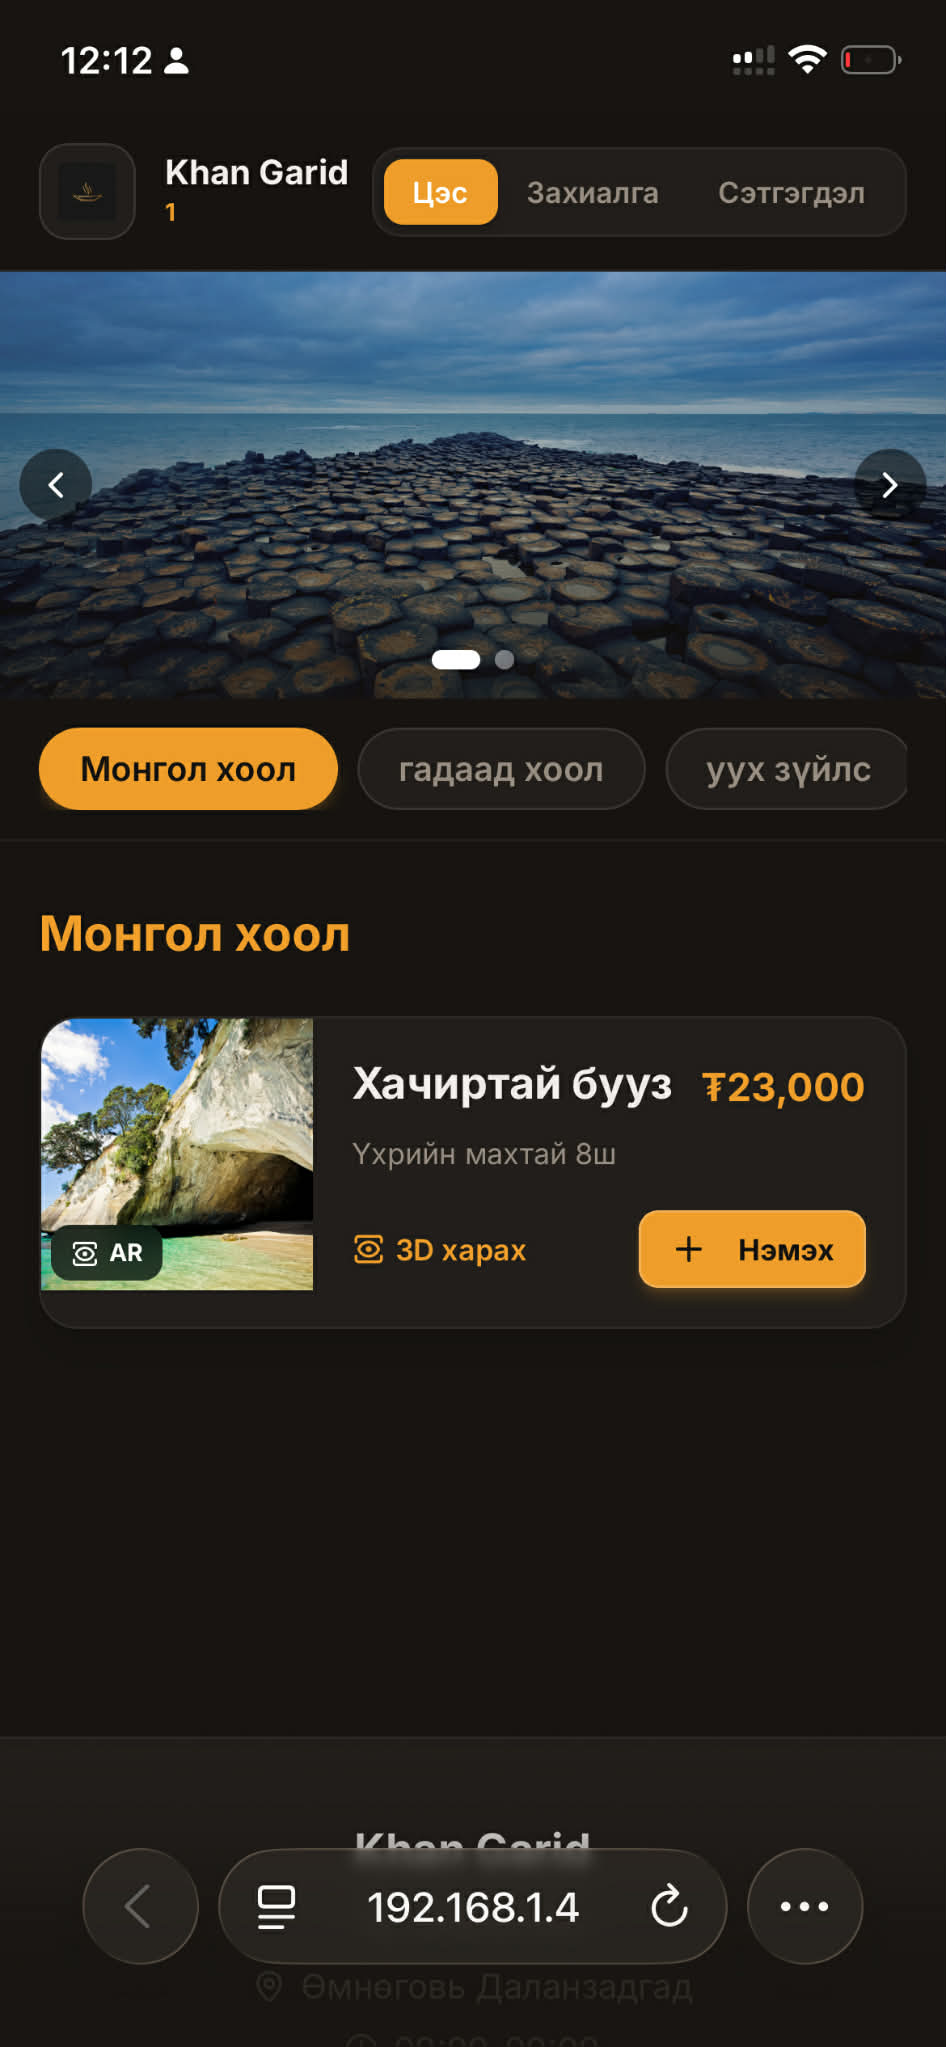
\includegraphics[width=0.45\textwidth]{Figures/guest-menu.png}
\caption{Зочны цэсийн дэлгэцийн дүрс (мобайл харагдац)}
\label{fig:guest-menu}
\end{figure}

\begin{figure}[htbp]
\centering
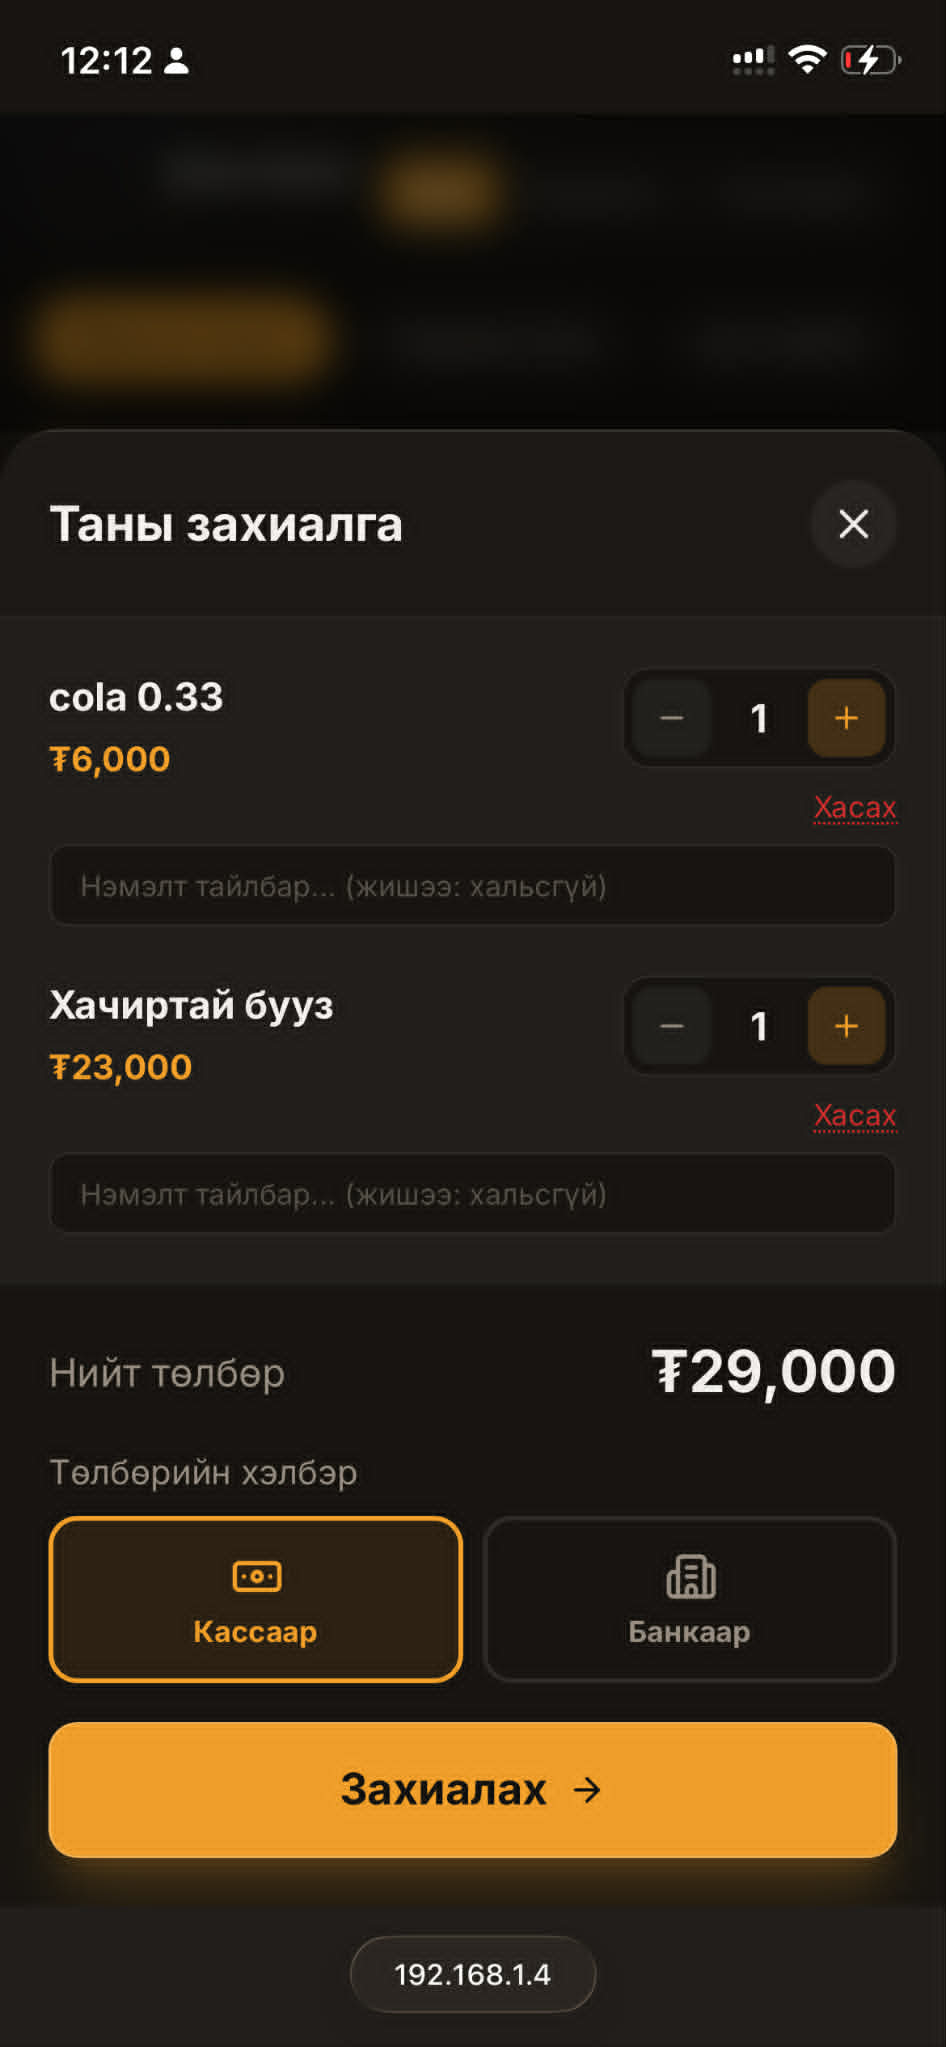
\includegraphics[width=0.45\textwidth]{Figures/guest-cart.png}
\caption{Зочны сагсны дэлгэц -- хоол сонгон захиалга өгөх}
\label{fig:guest-cart}
\end{figure}

\begin{figure}[htbp]
\centering
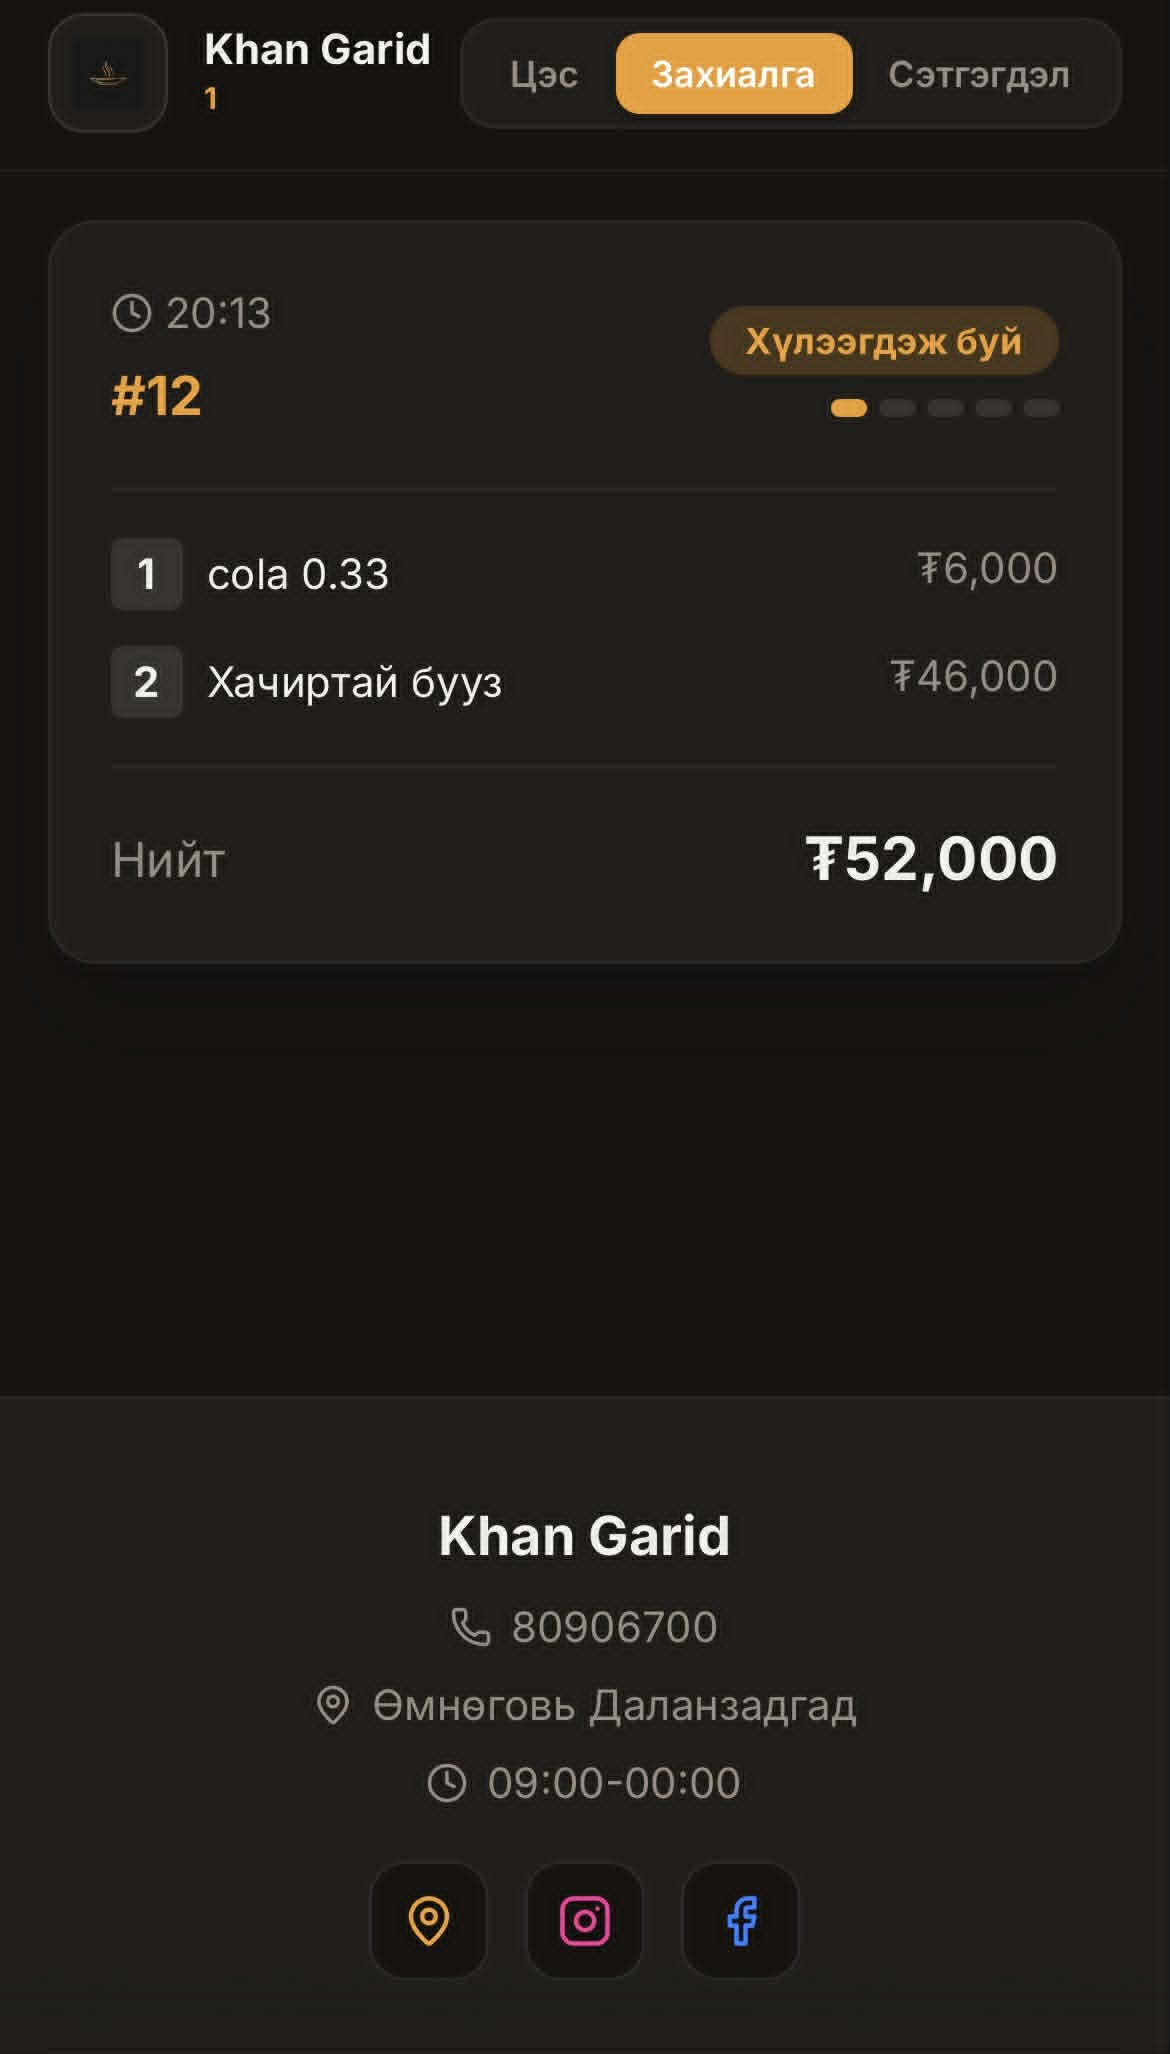
\includegraphics[width=0.45\textwidth]{Figures/guest-order-status.png}
\caption{Зочны захиалгын статус хянах дэлгэц}
\label{fig:guest-status}
\end{figure}

\subsection{Ажилтны удирдлагын самбар}

Ажилтны дэлгэц нь дараах модулиудтай:

\begin{itemize}
  \item \textbf{Захиалгын самбар}: Бодит цагийн захиалгын жагсаалт, статус шилжүүлгээ;
  \item \textbf{Ширээний удирдлага}: Ширээ нэмэх, засах, QR код хэвлэх;
  \item \textbf{Цэс удирдлага}: Ангилал, хоолны CRUD (Create, Read, Update, Delete);
  \item \textbf{Тайлан}: Өдрийн орлого, эрэлттэй хоол, ширээний статистик.
\end{itemize}

\begin{figure}[htbp]
\centering
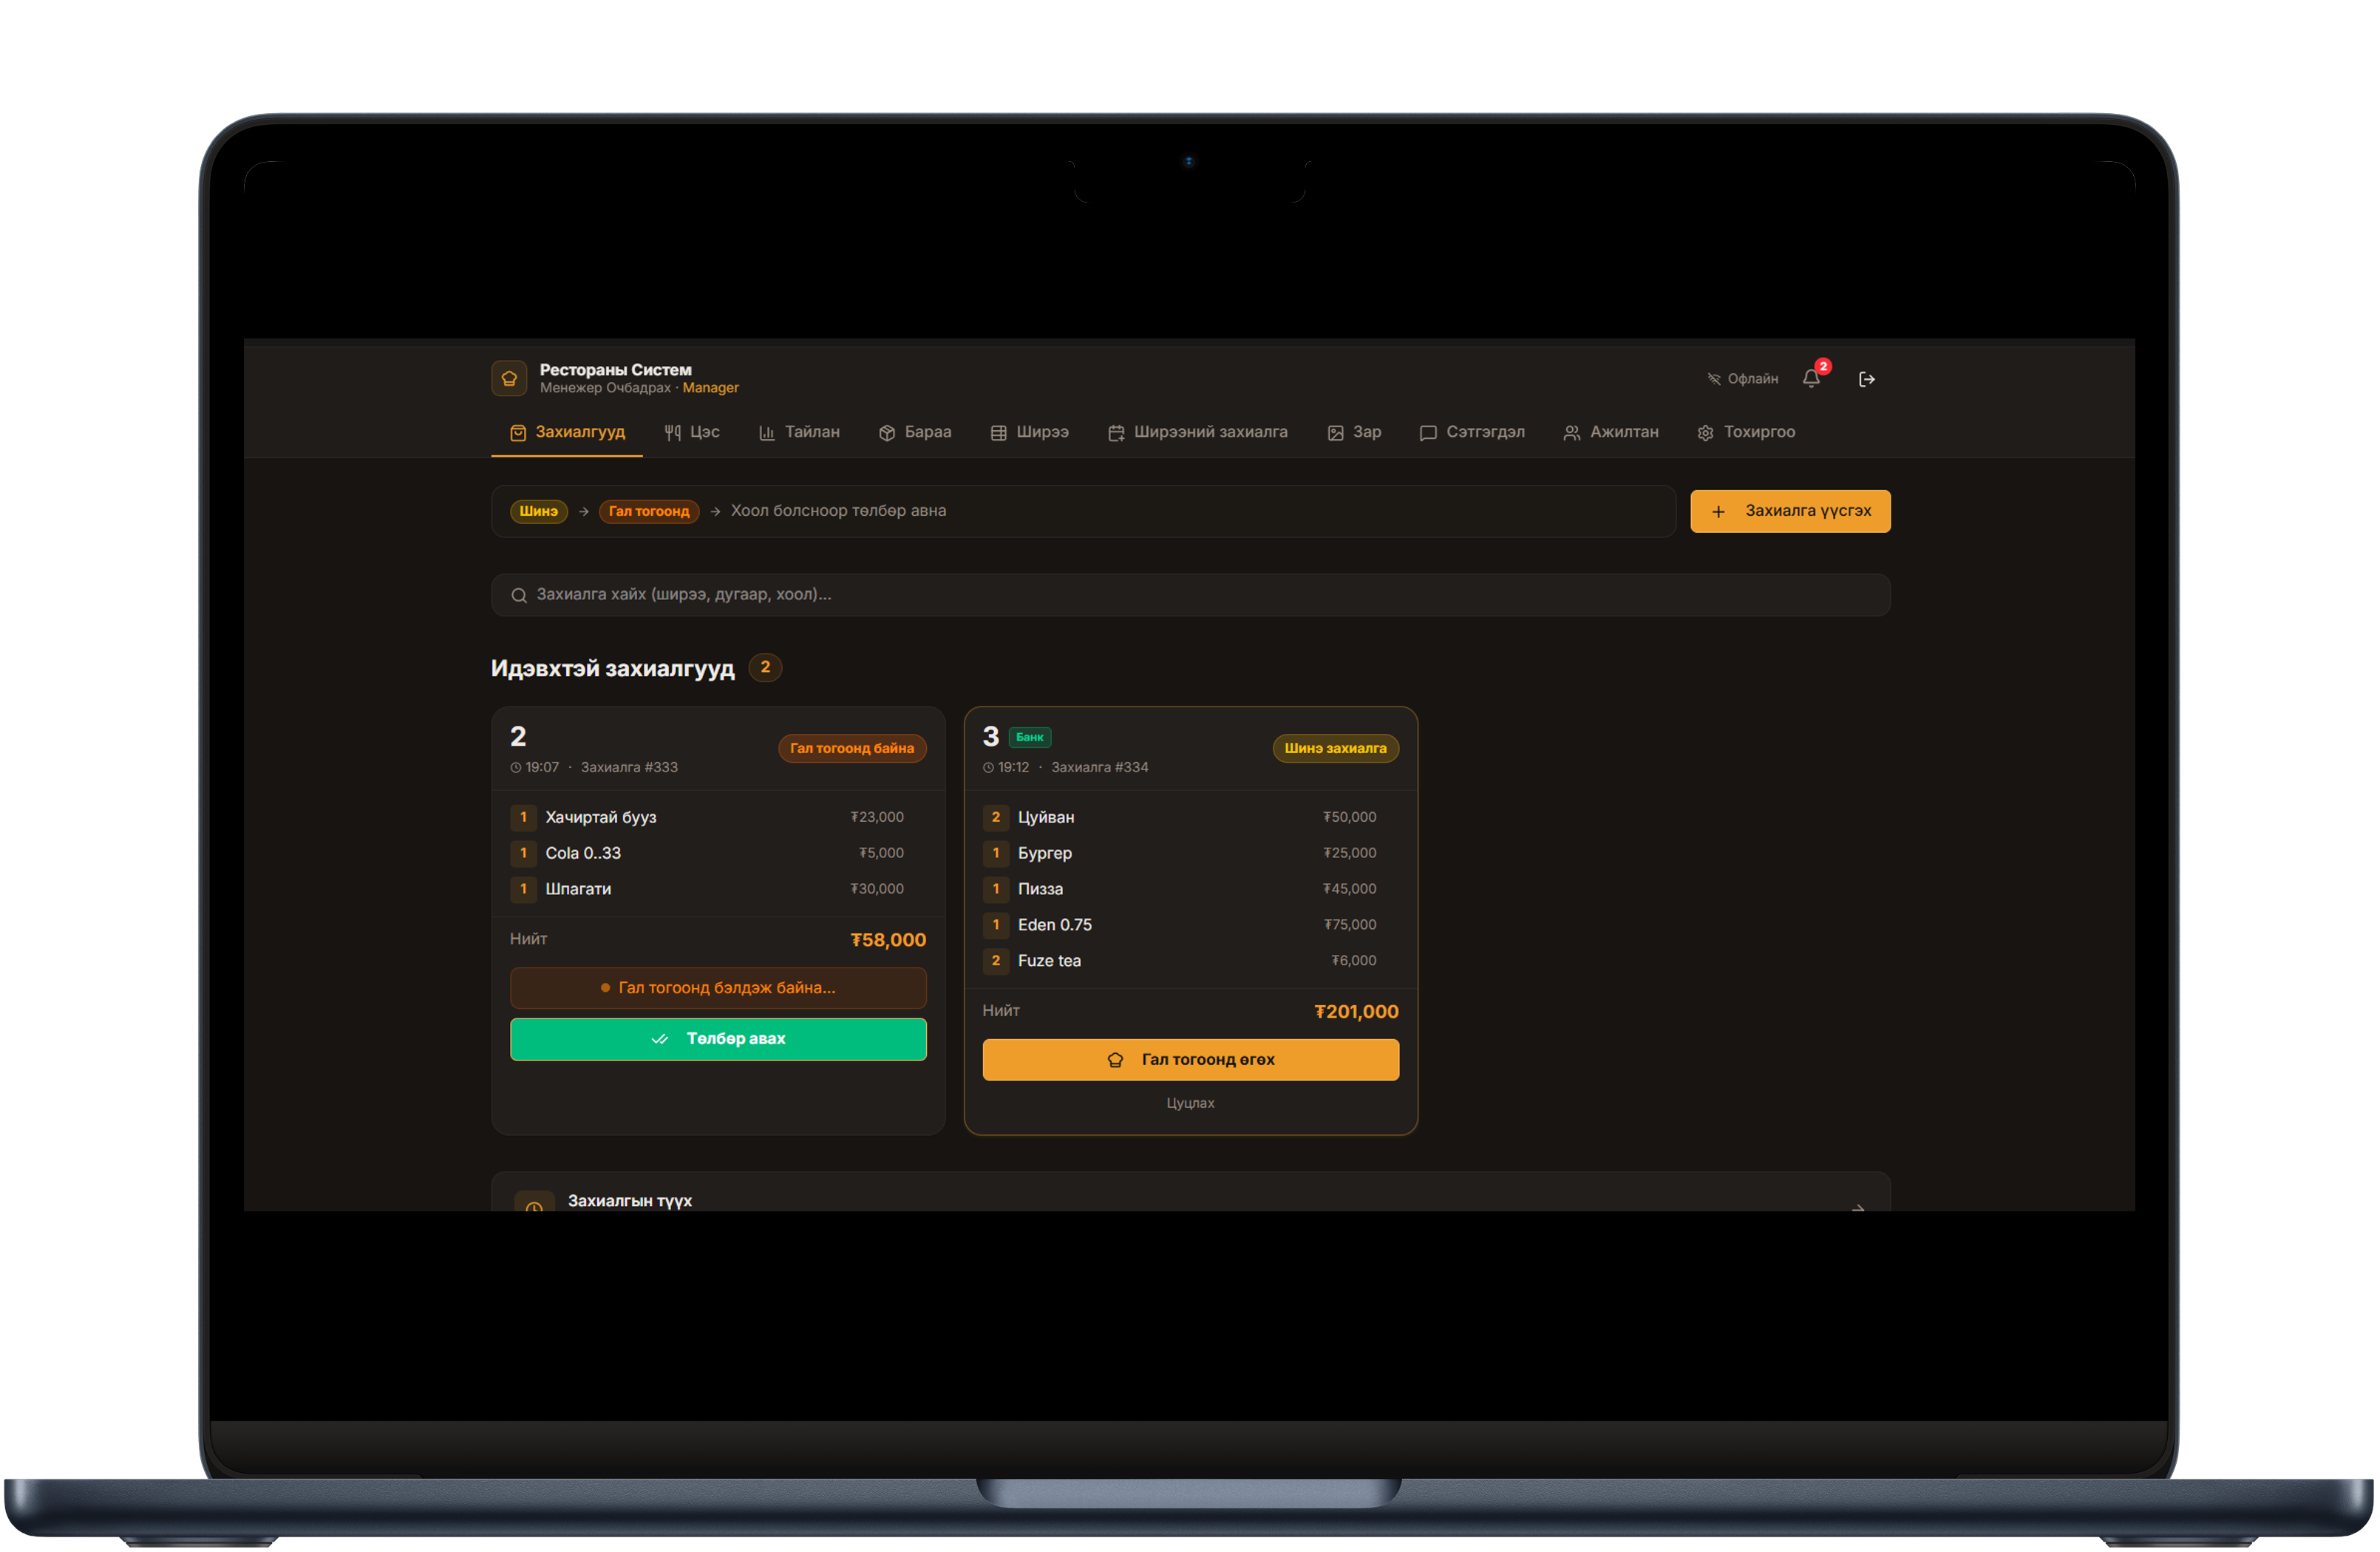
\includegraphics[width=0.95\textwidth]{Figures/staff-dashboard.png}
\caption{Ажилтны захиалгын удирдлагын самбар}
\label{fig:staff-dashboard}
\end{figure}

\begin{figure}[htbp]
\centering
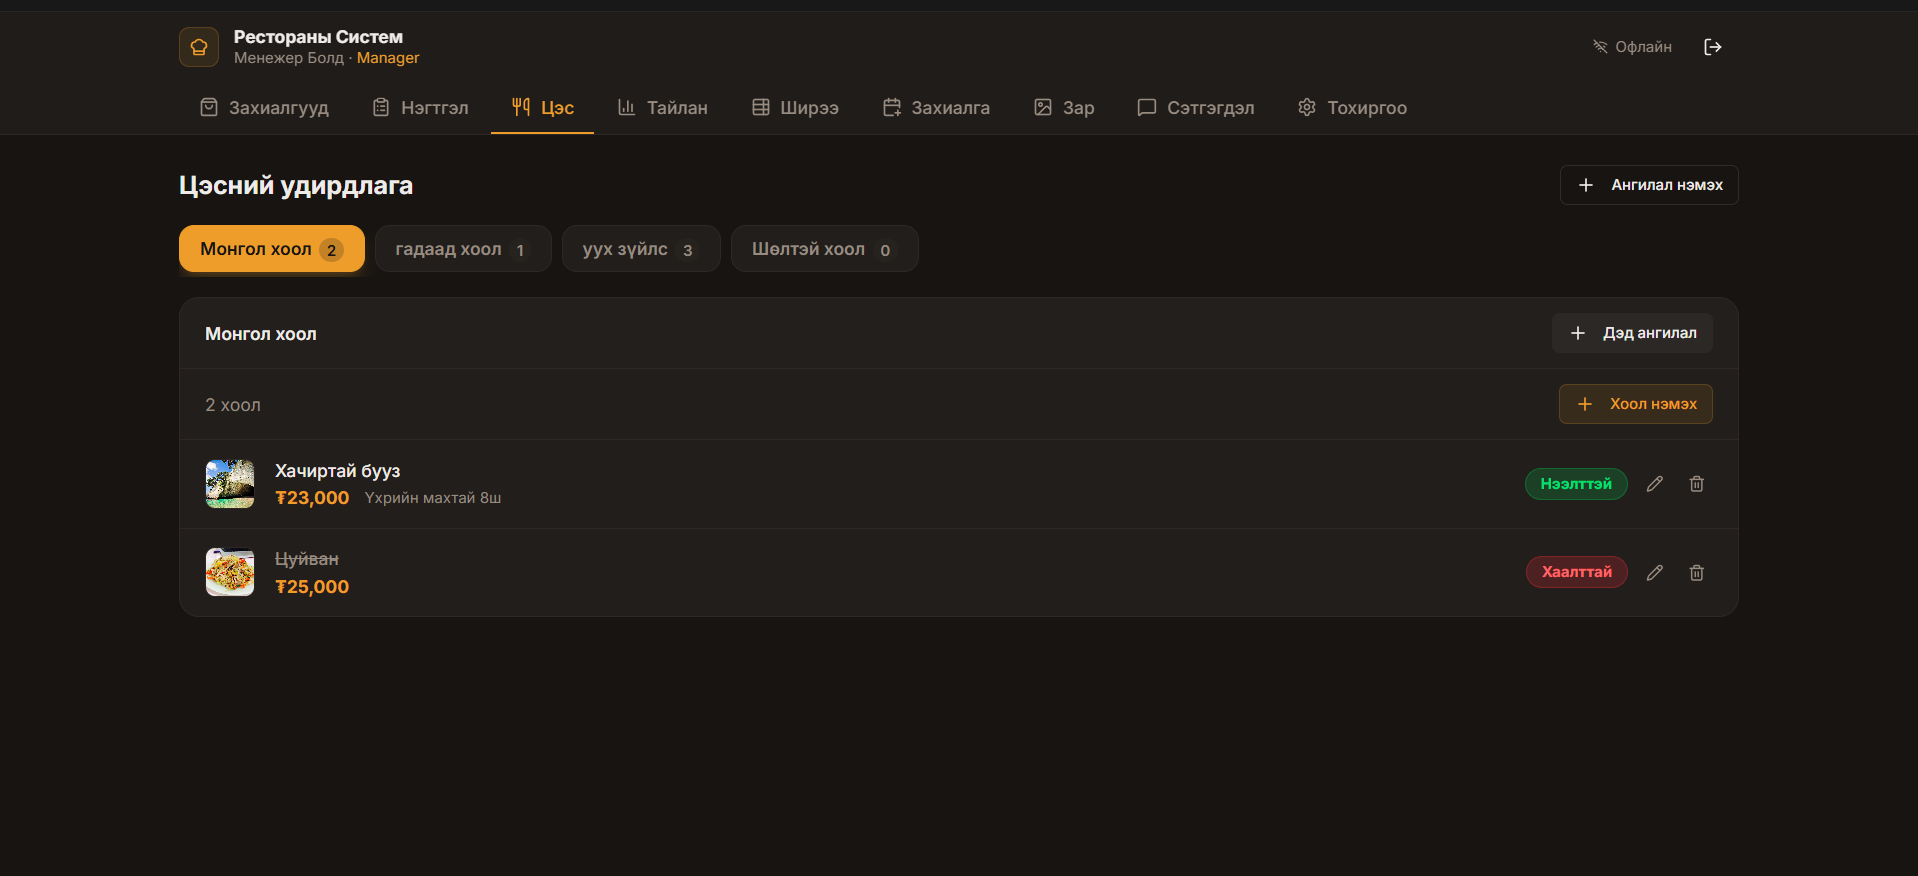
\includegraphics[width=0.95\textwidth]{Figures/staff-menu-manage.png}
\caption{Цэс удирдлагын дэлгэц -- хоол нэмэх, засах}
\label{fig:staff-menu}
\end{figure}

\begin{figure}[htbp]
\centering
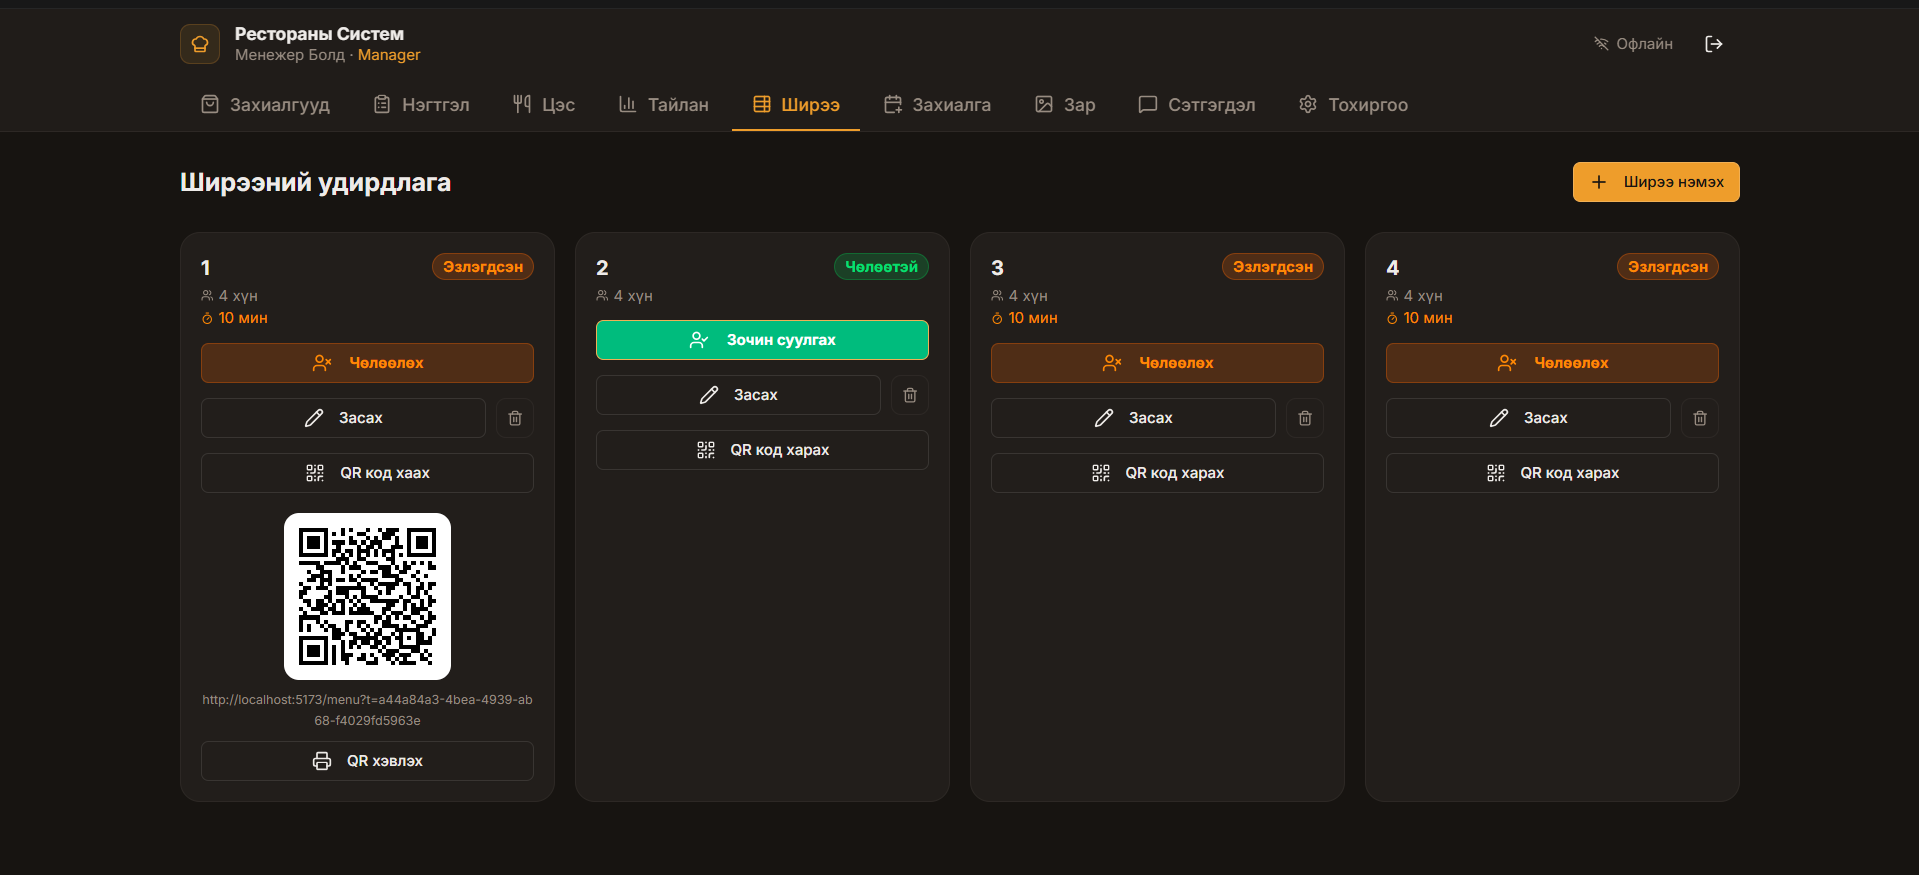
\includegraphics[width=0.95\textwidth]{Figures/staff-tables.png}
\caption{Ширээний удирдлага -- ширээ нэмэх, QR код хэвлэх}
\label{fig:staff-tables}
\end{figure}

\begin{figure}[htbp]
\centering
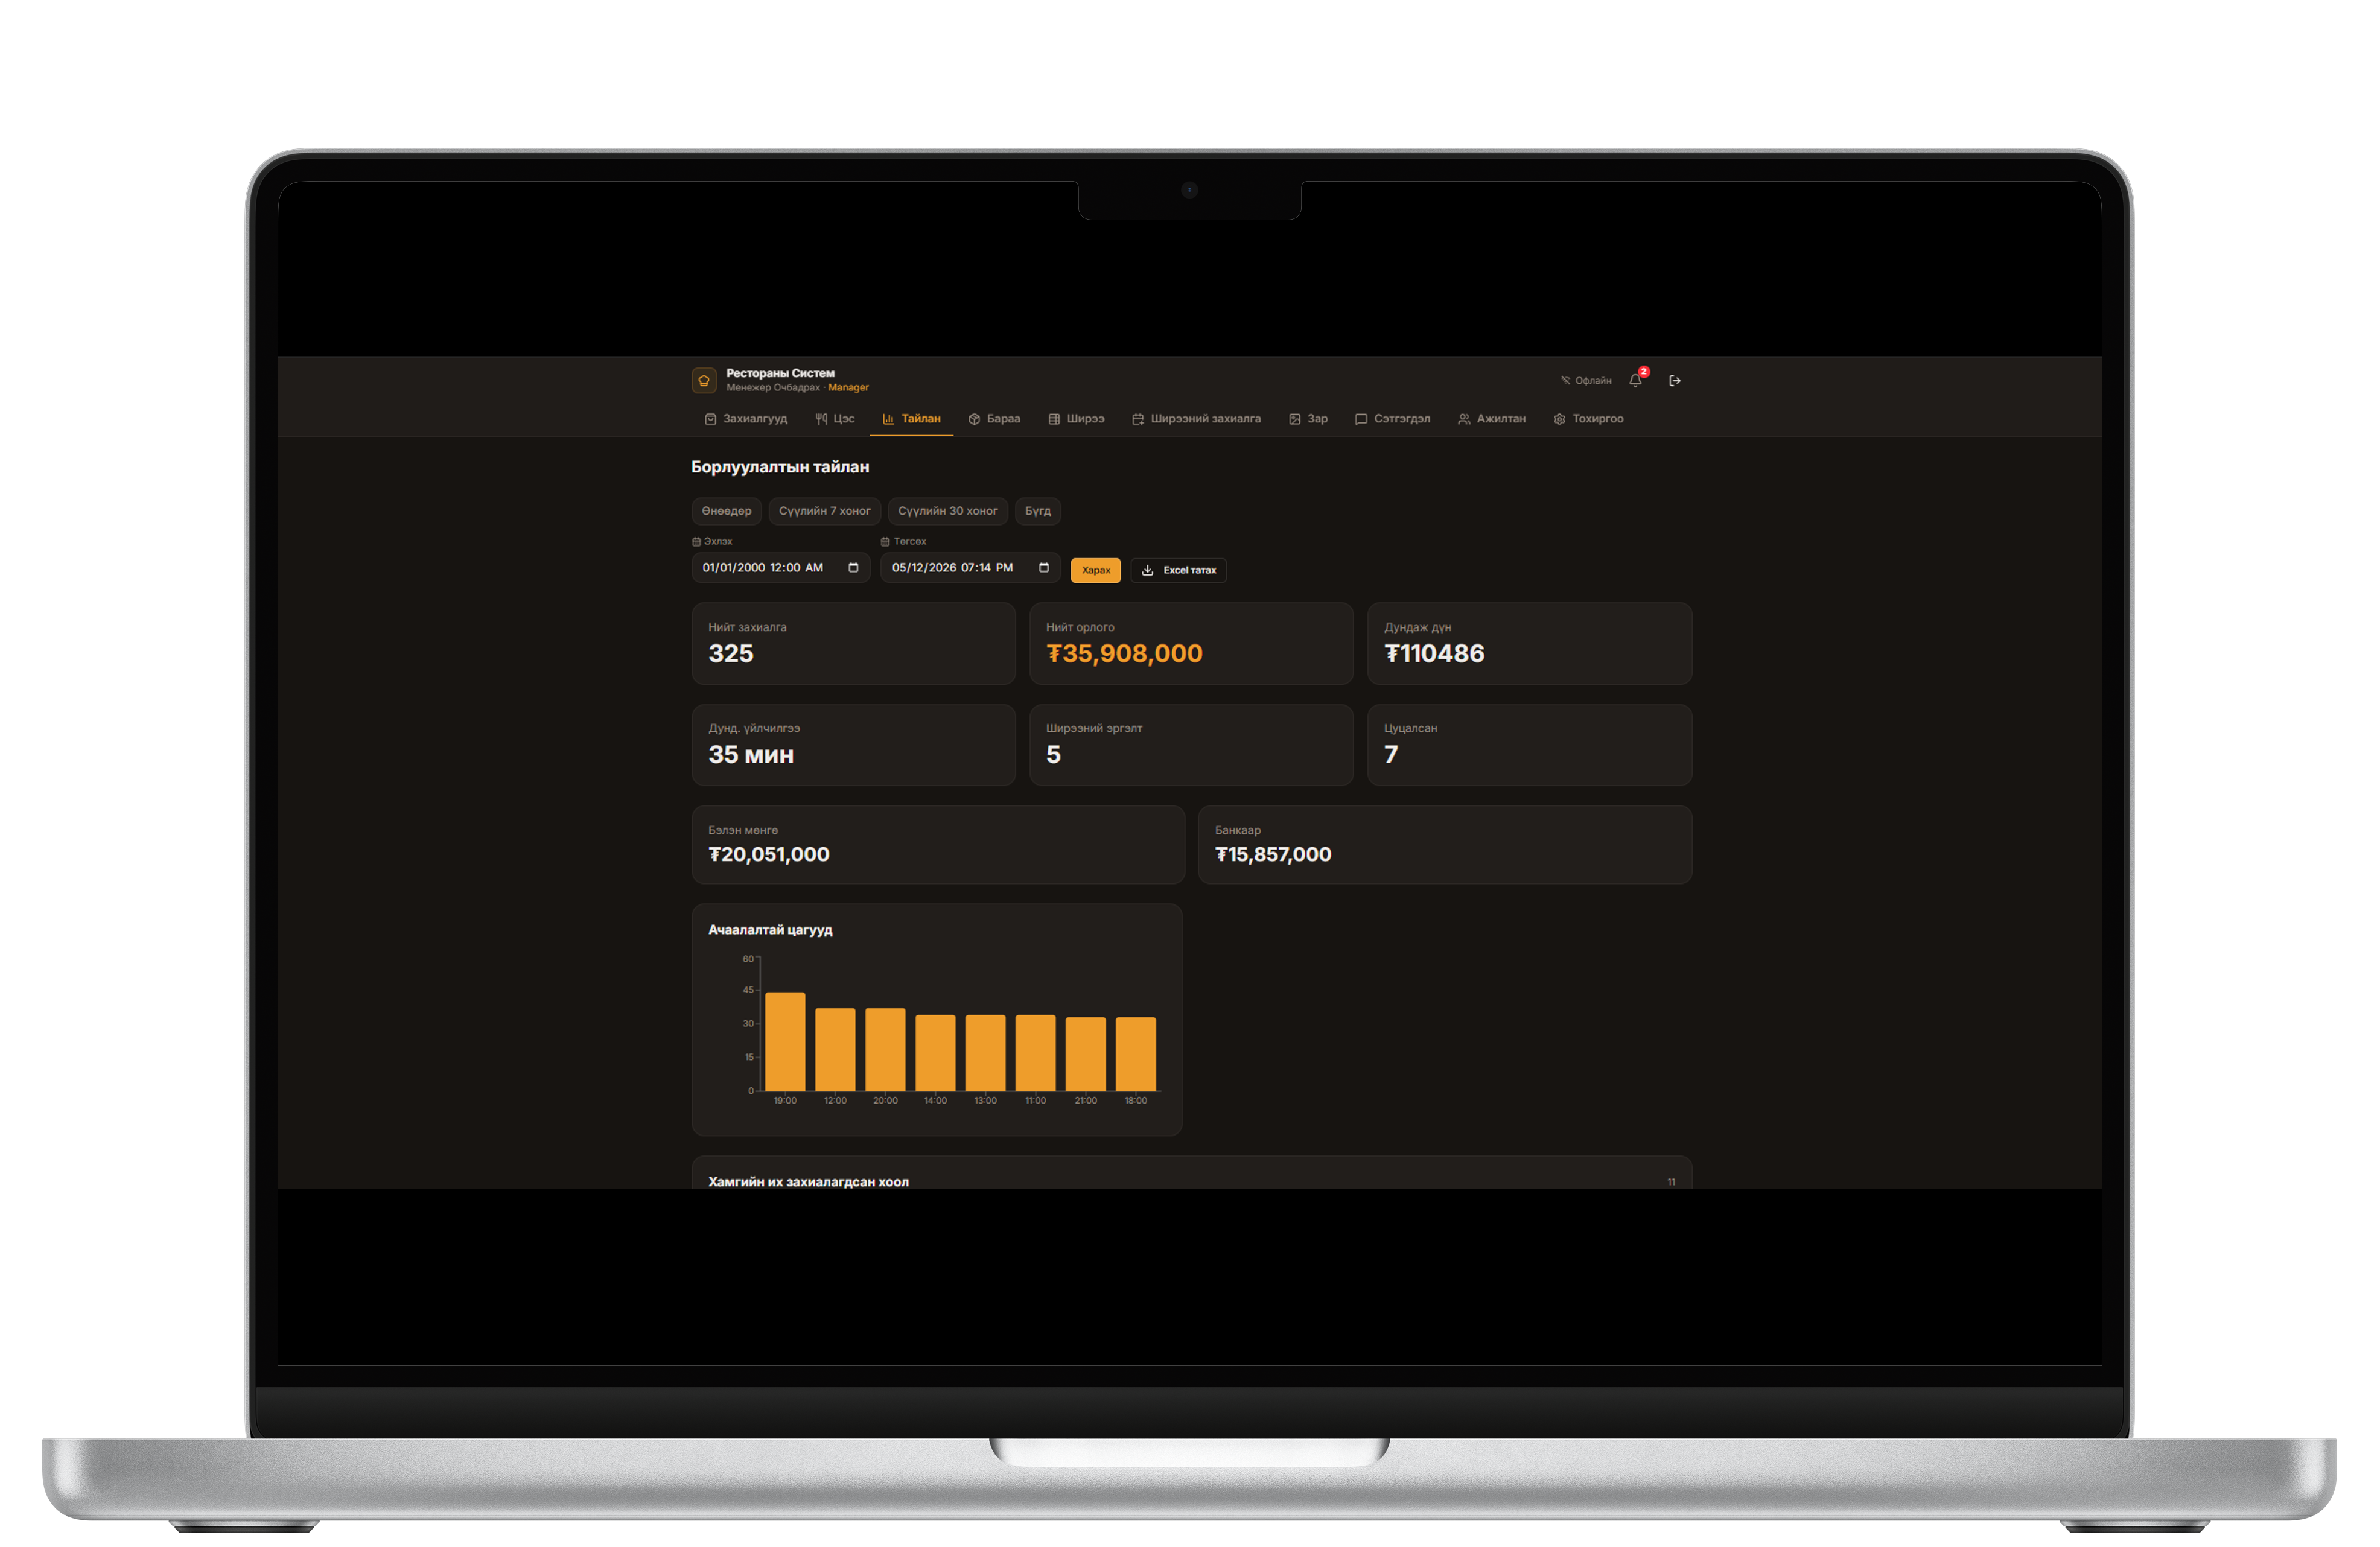
\includegraphics[width=0.95\textwidth]{Figures/staff-reports.png}
\caption{Тайлангийн дэлгэц -- өдрийн орлого, эрэлттэй хоол}
\label{fig:staff-reports}
\end{figure}

\begin{figure}[htbp]
\centering
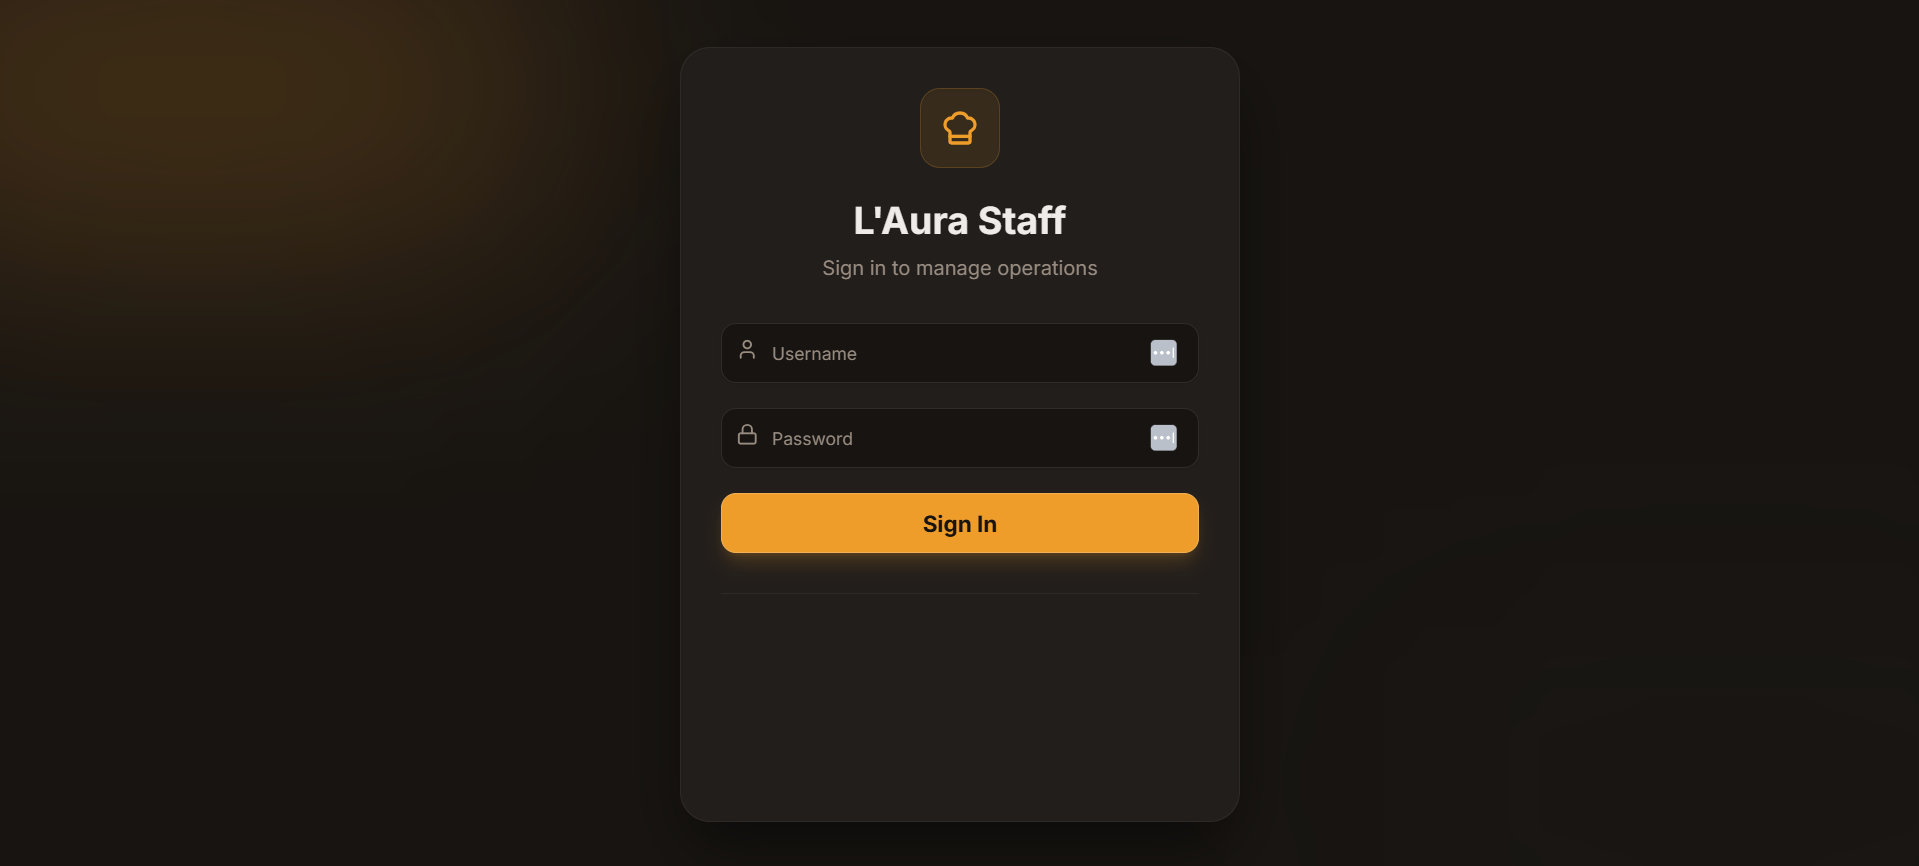
\includegraphics[width=0.95\textwidth]{Figures/login-page.png}
\caption{Ажилтны нэвтрэх дэлгэц}
\label{fig:login}
\end{figure}

\section{API жагсаалт}

Системийн REST API endpoint-уудыг бүлэг тус бүрээр (auth, menu, tables,
orders, inventory, reports, feedback, upload) нэгтгэн Хүснэгт~\ref{tab:api}
дээр харуулав.

\begin{longtable}{|c|l|l|p{5cm}|}
\caption{REST API endpoint-уудын жагсаалт} \label{tab:api} \\
\hline
\rowcolor{TableHdr}
\textcolor{white}{\textbf{No}} &
\textcolor{white}{\textbf{Метод}} &
\textcolor{white}{\textbf{Endpoint}} &
\textcolor{white}{\textbf{Тодорхойлолт}} \\ \hline
\endfirsthead
\hline
\rowcolor{TableHdr}
\textcolor{white}{\textbf{No}} &
\textcolor{white}{\textbf{Метод}} &
\textcolor{white}{\textbf{Endpoint}} &
\textcolor{white}{\textbf{Тодорхойлолт}} \\ \hline
\endhead

\multicolumn{4}{|l|}{\textbf{Auth}} \\ \hline
1 & POST & /api/auth/login & Нэвтрэх, JWT авах \\ \hline
\rowcolor{LightBlue}
2 & POST & /api/auth/register & Шинэ хэрэглэгч (manager-only) \\ \hline
3 & GET  & /api/auth/me & Одоогийн хэрэглэгчийн мэдээлэл \\ \hline
\multicolumn{4}{|l|}{\textbf{Menu}} \\ \hline
4 & GET  & /api/menu & Цэс (ангиллаар) \\ \hline
\rowcolor{LightBlue}
5 & GET  & /api/menu/categories & Ангиллын жагсаалт \\ \hline
6 & POST & /api/menu & Шинэ хоол нэмэх \\ \hline
\rowcolor{LightBlue}
7 & PUT  & /api/menu/:id & Хоолны мэдээлэл засах \\ \hline
8 & DELETE & /api/menu/:id & Хоол устгах \\ \hline
\multicolumn{4}{|l|}{\textbf{Tables}} \\ \hline
\rowcolor{LightBlue}
9 & GET  & /api/tables & Ширээний жагсаалт \\ \hline
10 & GET  & /api/tables/:token & QR token-оор ширээ \\ \hline
\rowcolor{LightBlue}
11 & POST & /api/tables & Шинэ ширээ \\ \hline
12 & PUT  & /api/tables/:id & Ширээ засах \\ \hline
\rowcolor{LightBlue}
13 & DELETE & /api/tables/:id & Ширээ устгах \\ \hline
14 & GET  & /api/tables/:id/qr & QR PNG татах \\ \hline
\multicolumn{4}{|l|}{\textbf{Orders}} \\ \hline
\rowcolor{LightBlue}
15 & GET  & /api/orders & Бүх захиалга \\ \hline
16 & GET  & /api/orders/:id & Нэг захиалгын дэлгэрэнгүй \\ \hline
\rowcolor{LightBlue}
17 & POST & /api/orders & Шинэ захиалга \\ \hline
18 & PATCH & /api/orders/:id & Статус шинэчлэх \\ \hline
\rowcolor{LightBlue}
19 & DELETE & /api/orders/:id & Захиалга цуцлах \\ \hline
\multicolumn{4}{|l|}{\textbf{Inventory}} \\ \hline
20 & GET  & /api/inventory & Нөөцийн бараа \\ \hline
\rowcolor{LightBlue}
21 & POST & /api/inventory & Шинэ бараа + менюнд нэмэх \\ \hline
22 & PATCH & /api/inventory/:id & Бараа засварлах \\ \hline
\rowcolor{LightBlue}
23 & DELETE & /api/inventory/:id & Бараа устгах (soft/hard) \\ \hline
\multicolumn{4}{|l|}{\textbf{Reports}} \\ \hline
24 & GET  & /api/reports/daily & Өдрийн орлого \\ \hline
\rowcolor{LightBlue}
25 & GET  & /api/reports/popular & Эрэлттэй хоол ТОП-10 \\ \hline
26 & GET  & /api/reports/low-stock & Доод хэмжээнд хүрсэн нөөц \\ \hline
\multicolumn{4}{|l|}{\textbf{Feedback ба бусад}} \\ \hline
\rowcolor{LightBlue}
27 & POST & /api/feedback & Зочны сэтгэгдэл илгээх \\ \hline
28 & GET  & /api/feedback & Менежерт сэтгэгдлүүд \\ \hline
\rowcolor{LightBlue}
29 & PATCH & /api/feedback/:id/read & Сэтгэгдэл уншсан тэмдэглэх \\ \hline
30 & POST & /api/upload & Зураг байршуулах (S3) \\ \hline

\end{longtable}

\section{Socket.IO үйл явдлууд}

Бодит цагийн харилцааны Socket.IO үйл явдлуудыг Хүснэгт~\ref{tab:socket} дээр
харуулав.

\begin{table}[htbp]
\caption{Socket.IO үйл явдлуудын жагсаалт}
\label{tab:socket}
\centering
\small
\begin{tabularx}{\textwidth}{|c|L|L|Y|}
\hline
\rowcolor{TableHdr}
\textcolor{white}{\textbf{No}} &
\textcolor{white}{\textbf{Үйл явдал}} &
\textcolor{white}{\textbf{Чиглэл}} &
\textcolor{white}{\textbf{Тодорхойлолт}} \\ \hline
1 & connect & Клиент $\to$ Сервер & Socket холболт тогтоох \\ \hline
\rowcolor{LightBlue}
2 & join\_room & Клиент $\to$ Сервер & restaurant\_1 эсвэл ширээний room-д нэгдэх \\ \hline
3 & new\_order & Сервер $\to$ Ажилтан & Шинэ захиалга broadcast \\ \hline
\rowcolor{LightBlue}
4 & order\_update & Сервер $\to$ Клиент & Захиалгын статус шинэчлэлт \\ \hline
5 & order\_confirmed & Сервер $\to$ Зочин & Захиалга баталгаажсан мэдэгдэл \\ \hline
\rowcolor{LightBlue}
6 & table\_update & Сервер $\to$ Клиент & Ширээний статус шинэчлэлт \\ \hline
7 & low\_stock & Сервер $\to$ Менежер & Нөөц доод хэмжээнд хүрсэн \\ \hline
\rowcolor{LightBlue}
8 & new\_feedback & Сервер $\to$ Менежер & Зочноос сэтгэгдэл ирсэн \\ \hline
9 & disconnect & Клиент $\to$ Сервер & Холболт тасрах \\ \hline
\end{tabularx}
\end{table}

\section{Гүйцэтгэлийн туршилт}

\subsection{k6 ачааллын туршилт}

Системийн гүйцэтгэлийг k6 ачааллын туршилтын хэрэгслээр шалгасан. Туршилтын
тохиргоо: 200 виртуал хэрэглэгч (VU), 5 минутын хугацаа, ramp-up 30 секунд.

\begin{table}[htbp]
\caption{k6 ачааллын туршилтын үр дүн}
\label{tab:k6}
\centering
\small
\begin{tabularx}{\textwidth}{|L|Y|Y|Y|}
\hline
\rowcolor{TableHdr}
\textcolor{white}{\textbf{Endpoint}} &
\textcolor{white}{\textbf{Дундаж (мс)}} &
\textcolor{white}{\textbf{p95 (мс)}} &
\textcolor{white}{\textbf{p99 (мс)}} \\ \hline
GET /api/menu & 45 & 89 & 134 \\ \hline
\rowcolor{LightBlue}
GET /api/tables/:token & 38 & 72 & 112 \\ \hline
POST /api/orders & 120 & 198 & 287 \\ \hline
\rowcolor{LightBlue}
PATCH /api/orders/:id & 85 & 156 & 223 \\ \hline
GET /api/reports/daily & 156 & 245 & 312 \\ \hline
\rowcolor{LightBlue}
WebSocket мессеж & 45 & 78 & 98 \\ \hline
\end{tabularx}
\end{table}

Туршилтын үр дүнгээс харахад бүх endpoint-ийн дундаж хариу хугацаа 200 мс-ээс бага
байгаа нь функционал бус шаардлагыг (Хүснэгт~\ref{tab:nfr_perf}) бүрэн хангаж байна.
WebSocket мессежийн дамжуулалт 45 мс дунджаар буюу 100 мс-ээс бага шаардлагыг давж
хангасан.

\subsection{Ачааллын графикийн дүн шинжилгээ}

200 VU-ийн ачаалалд серверийн CPU ашиглалт дунджаар 35\%, санах ой (RAM) 512 MB
орчим байсан бөгөөд энэ нь серверийн доод шаардлага (2 CPU, 4 GB RAM)-ийн хүрээнд
тогтвортой ажиллаж байгааг харуулж байна.

\section{SUS (System Usability Scale) үнэлгээ}

Системийн хэрэглэхэд хялбар байдлыг үнэлэхийн тулд 28 хэрэглэгч (20 зочин + 4
кассир + 4 менежер)-ээр SUS стандарт асуулгын аргачлалаар үнэлгээ хийлгэсэн.

SUS нь John Brooke-ийн 1986 онд боловсруулсан 10 асуулт бүхий стандартчилсан
хэрэглэгчийн сэтгэл ханамжийн арга бөгөөд 0--100 оноогоор дүгнэгддэг~\cite{brooke1996}.

\begin{table}[htbp]
\caption{SUS үнэлгээний үр дүн}
\label{tab:sus}
\centering
\small
\begin{tabularx}{\textwidth}{|c|L|Y|}
\hline
\rowcolor{TableHdr}
\textcolor{white}{\textbf{No}} &
\textcolor{white}{\textbf{Асуулт}} &
\textcolor{white}{\textbf{Дундаж оноо}} \\ \hline
1 & Би энэ системийг байнга ашиглахыг хүснэ & 4.1 \\ \hline
\rowcolor{LightBlue}
2 & Систем хэт нарийн төвөгтэй санагдсан & 1.6 \\ \hline
3 & Системийг ашиглахад хялбар байсан & 4.3 \\ \hline
\rowcolor{LightBlue}
4 & Системийг ашиглахын тулд тусламж хэрэгтэй & 1.4 \\ \hline
5 & Системийн функцууд сайн нэгтгэгдсэн & 4.0 \\ \hline
\rowcolor{LightBlue}
6 & Системд хэт их зөрчил байна & 1.5 \\ \hline
7 & Ихэнх хүмүүс хурдан сурч чадна & 4.4 \\ \hline
\rowcolor{LightBlue}
8 & Систем ашиглахад маш их төвөгтэй & 1.3 \\ \hline
9 & Системийг ашиглахдаа итгэлтэй байсан & 4.2 \\ \hline
\rowcolor{LightBlue}
10 & Системийг ашиглахаас өмнө олон зүйл сурах хэрэгтэй & 1.5 \\ \hline
\multicolumn{2}{|r|}{\textbf{Нийт SUS оноо}} & \textbf{84.2} \\ \hline
\end{tabularx}
\end{table}

SUS оноо 84.2 нь ``Маш сайн'' (Excellent) зэрэглэлд хамаарах бөгөөд Bangor нарын
ангиллаар A зэрэглэлд хамаарна~\cite{bangor2009}. Энэ нь системийн хэрэглэхэд
хялбар, ойлгомжтой болохыг баталж байна.

\section{Уламжлалт аргатай харьцуулсан үр дүн}

Системийн үр дүнг уламжлалт рестораны үйлчилгээний аргатай харьцуулахын тулд
ижил нөхцөлд туршилт хийсэн (Хүснэгт~\ref{tab:compare_trad}).

\begin{table}[htbp]
\caption{Уламжлалт арга ба QR системийн харьцуулалт}
\label{tab:compare_trad}
\centering
\small
\begin{tabularx}{\textwidth}{|L|Y|Y|Y|}
\hline
\rowcolor{TableHdr}
\textcolor{white}{\textbf{Шалгуур}} &
\textcolor{white}{\textbf{Уламжлалт}} &
\textcolor{white}{\textbf{QR систем}} &
\textcolor{white}{\textbf{Өөрчлөлт}} \\ \hline
Захиалга өгөх хугацаа & 4.2 мин & 1.6 мин & $-$62\% \\ \hline
\rowcolor{LightBlue}
Захиалгын алдааны хувь & 8.0\% & 0.5\% & $-$94\% \\ \hline
Гал тогоонд хүрэх хугацаа & 4.2 мин & 0.045 мин & $-$99\% \\ \hline
\rowcolor{LightBlue}
Нэг ажилтан хариуцах ширээ & 8--10 & 20--30 & $+$150\% \\ \hline
Олон хэлний дэмжлэг & Хязгаартай & Бүрэн & -- \\ \hline
\rowcolor{LightBlue}
Тайлан, нэгтгэл & Гар ажиллагаа & Автомат & -- \\ \hline
\end{tabularx}
\end{table}

Хүснэгт~\ref{tab:compare_trad}-с харахад QR системийг нэвтрүүлснээр:
\begin{itemize}
  \item Захиалга өгөх хугацаа 62\%-иар буурсан;
  \item Захиалгын алдааны хувь 94\%-иар буурсан;
  \item Захиалга гал тогоонд хүрэх хугацаа 99\%-иар буурсан;
  \item Нэг ажилтны хариуцах ширээний тоо 150\%-иар нэмэгдсэн.
\end{itemize}

\section{Хэрэгжүүлсэн системийн эх кодын жишээ}

\subsection{Express.js серверийн үндсэн тохиргоо}

\begin{lstlisting}[language=JavaScript, caption={Express серверийн эхлүүлэх код}, label={lst:server}]
import express from 'express';
import { createServer } from 'http';
import { Server } from 'socket.io';
import cors from 'cors';

const app = express();
const server = createServer(app);
const io = new Server(server, {
  cors: { origin: '*' }
});

app.use(cors());
app.use(express.json());

// Socket.IO connection handler
io.on('connection', (socket) => {
  socket.on('join_room', (tableId) => {
    socket.join(`table_${tableId}`);
  });

  socket.on('new_order', (order) => {
    io.to('staff').emit('order_update', order);
  });
});

server.listen(8080, () => {
  console.log('Server running on port 8080');
});
\end{lstlisting}

\subsection{Drizzle ORM Schema тодорхойлолт}

\begin{lstlisting}[language=JavaScript, caption={Drizzle ORM schema жишээ}, label={lst:drizzle}]
import { pgTable, serial, varchar, integer,
  numeric, boolean, timestamp, uuid } from 'drizzle-orm/pg-core';

export const tables = pgTable('tables', {
  id: serial('id').primaryKey(),
  name: varchar('name', { length: 20 }).notNull(),
  qrToken: uuid('qr_token').defaultRandom().unique(),
  capacity: integer('capacity').default(4),
  status: varchar('status', { length: 20 })
    .default('available'),
});

export const menuItems = pgTable('menu_items', {
  id: serial('id').primaryKey(),
  categoryId: integer('category_id')
    .references(() => menuCategories.id),
  name: varchar('name', { length: 200 }).notNull(),
  price: numeric('price', { precision: 10, scale: 2 })
    .notNull(),
  imageUrl: varchar('image_url'),
  available: boolean('available').default(true),
});
\end{lstlisting}

\section{Бүлгийн дүгнэлт}

Энэхүү бүлэгт системийн 4 давхаргат архитектурыг тодорхойлж, компонент болон
хэрэгжүүлэлтийн диаграмаар дэлгэрэнгүй дүрсэлсэн. 9 хүснэгт бүхий ER диаграм
болон SQL schema-г нарийвчлан боловсруулж, \texttt{inventory\_items},
\texttt{table\_sessions}, \texttt{feedback} гэх системийн өргөтгөсөн функцүүдийг
тусгасан. Захиалгын статусын шилжилтийн state machine диаграм, үндсэн захиалга
болон нөөц хасалтын дараалал, JWT нэвтрэх сайд зэрэг 4 дарааллын диаграм,
swimlane-тэй үйл ажиллагааны диаграмаар системийн урсгалыг бүрэн загварчилсан.
Нийт 30 REST API endpoint-ийг 8 бүлэгт хувааж тодорхойлон 9 Socket.IO үйл явдлыг
хэрэгжүүлсэн. k6 ачааллын туршилтаар системийн гүйцэтгэл шаардлагыг хангаж
байгааг баталж, SUS үнэлгээгээр 84.2 оноо авсан нь ``Маш сайн'' зэрэглэлд
хамаарч байгааг тогтоосон. Уламжлалт аргатай харьцуулахад захиалгын хугацаа 62\%,
алдааны хувь 94\%-иар буурсан гэсэн тодорхой үр дүн гарсан.
